\documentclass[IB,BIB]{TFUOC}%IB: CASTELLANO, CAT: CATALÁN, ENG: ANGLÈS

%Introducción de datos del trabajo
% \title{$title$} %Título del trabajo completo y tan largo como sea necesario
\title{Assessing the properties of asymptotic \break PERMANOVA test through comprehensive \break simulations in the context of genetic studies} %Título del trabajo completo y tan largo como sea necesario
\titcrt{Assessing the properties of asymptotic \break PERMANOVA through simulations} %Título corto que aparecerá a la cabecera
\author{$author$} %Nombre Estudiando Estudiante
\date{$date$}


\nomPDC{$nomPDC$} %Nombre Tutor Tutora
\nomPRA{$nomPRA$} %Nombre Profesorado Responsable
\titulac{$titulac$} %Máster en XXX
\area{$area$} %Área del trabajo
\idioma{$idioma$} %Castellano
\credits{$credits$} %15
\parcla{$parcla$} %palabra, clave, trabajo


\licenc{$licenc$}
% \licenc{ccByNcNd}
% \licenc{ccByNcSa}
% \licenc{ccByNc}
% \licenc{ccByNd}
% \licenc{ccBySa}
% \licenc{ccBy}
% \licenc{GNU}
% \licenc{copyright}
%Posibles licencias
%ccByNcNd
%ccByNcSa
%ccByNc
%ccByNd
%ccBySa
%ccBy
%GNU
%copyright


% Resumen en el idioma del documento
\abstractidioma{$abstractesp$}
% Máximo 250 palabras, con la finalidad, contexto de aplicación, metodología, resultados y conclusiones del trabajo.

% Resumen en inglés
\abstractenglish{$abstracteng$}
% A maximum of 250 words, detailing the purpose, contexto of application, methodology, results and conclusiones of the work.

% Añadir una Lista de Ecuaciones
\usepackage{tocloft}
\newcommand{\listequationsname}{Índice de Ecuaciones}
\newlistof{myequations}{equ}{\listequationsname}
\newcommand{\myequations}[1]{
\refstepcounter{myequations}%
\par\noindent\textbf{Equation \themyequations. #1}
\addcontentsline{equ}{myequations}{\protect\numberline{\thechapter.\themyequations}#1}\par}
\setlength{\cftmyequationsnumwidth}{2.5em} % Ancho del número de ecuación en la Lista de ecuaciones

% Paquetes a cargar
\usepackage{float}

\usepackage{hyperref}
\hypersetup{
    bookmarks=true,         % show bookmarks bar?
    unicode=false,          % non-Latin characters in Acrobat’s bookmarks
    %pdftoolbar=true,        % show Acrobat’s toolbar?
    %pdfmenubar=true,        % show Acrobat’s menu?
    pdffitwindow=false,     % window fit to page when opened
    pdfstartview={FitH},    % fits the width of the page to the window
    pdftitle={My title},    % title
    pdfauthor={Author},     % author
    pdfsubject={Subject},   % subject of the document
    pdfcreator={Creator},   % creator of the document
    pdfproducer={Producer}, % producer of the document
    pdfkeywords={keyword1, key2, key3}, % list of keywords
    pdfnewwindow=true,      % links in new PDF window
    colorlinks=true,       % false: boxed links; true: colored links
    linkcolor=[RGB]{106,90,205},          % color of internal links (change box color with linkbordercolor)
    citecolor=[RGB]{204 0 0},        % color of links to bibliography
    filecolor=[RGB]{147,112,219},         % color of file links
    urlcolor=[RGB]{72,61,139}        % color of external links
}

\usepackage{multicol}
\usepackage{lipsum}
\usepackage{tikz}
\usepackage{amsmath}
\usepackage{siunitx}
\usepackage[T1]{fontenc}
\usepackage{pdflscape}
\usepackage[notindex]{tocbibind}

% Glosario
% \usepackage{glossaries} % Glosario y acrónimos juntos
% \usepackage[acronym]{glossaries} % Glosario y acrónimos separados
% \usepackage[xindy]{glossaries} % Glosario y acrónimos separados
% \usepackage[toc]{glossaries} % Glosario y acrónimos juntos + TOC
\usepackage[automake, toc]{glossaries} % Para no usar makeglossaries
%%%%%%%%%%%%%%%%
% Glosario TFM %
%%%%%%%%%%%%%%%%

\makeglossaries

% Definición de términos
%%%%%%%%%%%%%%%%%%%%%%%%

% \newglossaryentry{ex}{name={sample},description={an example}}

\newglossaryentry{estadística multivariante}
  {name=estadística multivariante,
   description={La estadística multivariante o multivariada es una rama de las estadísticas que abarca la observación y el análisis simultáneos de más de una variable respuesta. La aplicación de la estadística multivariante es llamada análisis estadístico multivariante}
  }
  
\newglossaryentry{MANOVA}
  {name=MANOVA,
   description={En estadística el análisis multivariante de la varianza (Multivariate analysis of variance) es una extensión del análisis de la varianza o ANOVA para cubrir los casos donde hay más de una variable dependiente que no pueden ser combinadas de manera simple. Además de identificar si los cambios en las variables independientes tienen efectos significativos en las variables dependientes, la técnica también intenta identificar las interacciones entre las variables independientes y su grado de asociación con las dependientes}
  }

\newglossaryentry{PERMANOVA}
  {name=PERMANOVA,
   description={El análisis multivariante de la varianza con permutaciones (Permutational multivariate analysis of variance, PERMANOVA) es una prueba de permutación estadística multivariada no paramétrica. Se utiliza para comparar grupos de objetos y probar la hipótesis nula de que los centroides y la dispersión de los grupos definidos por el espacio de medida son equivalentes para todos los grupos. Un rechazo de la hipótesis nula significa que el centro y/o la dispersión de los objetos es diferente entre los grupos. De esta manera, la prueba se basa en el cálculo previo de la distancia entre cualesquier dos objetos incluidos en el experimento}
  }
  
\newglossaryentry{SNPs}
  {name=SNPs,
   description={Un polimorfismo puntual, también denominado de un solo nucleótido o SNP (Single Nucleotide Polymorphism, pronunciado snip), es una variación en la secuencia de ADN que afecta a una sola base (adenina (A), timina (T), citosina (C) o guanina (G)) de una secuencia del genoma. Sin embargo, generalmente se considera que cambios de unos pocos nucleótidos, como también pequeñas inserciones y deleciones (indels) pueden ser consideradas como SNP. Una de estas variaciones debe darse al menos en un 1 \% de la población para ser considerada como un SNP. Si no se llega al 1 \% no se considera SNP y sí una mutación puntual. En ocasiones estas variaciones de nucleótido único se asocian a otro término conocido como SNV (Single Nucleotide Variant), que a diferencia de los SNPs carece de limitaciones de frecuencia}
  }
  
\newglossaryentry{GWAS}
  {name=GWAS,
   description={En genética, un estudio de asociación del genoma completo (Genome-wide association study) o WGAS (Whole genome association study) es un análisis de una variación genética a lo largo de todo el genoma humano con el objetivo de identificar su asociación a un rasgo observable. Los GWAS suelen centrarse en asociaciones entre los polimorfismos de un solo nucleótido (SNPs) y rasgos como las principales enfermedades}
  }
  
\newglossaryentry{sQTLs}
  {name=sQTLs,
   description={Los \textit{Splicing quantitative trait loci} (sQTLs o splicing QTLs) son los loci que regulan el splicing alternativo del ARNm. Se pueden detectar utilizando datos de RNA-seq. Se han desarrollado diversos métodos para descubrir sQTLs, entre los que se incluyen: LeafCutter, Altrans, Cufflinks, y MISO}
  }
  
\newglossaryentry{RNA-seq}
  {name=RNA-seq,
   description={La secuenciación de ARN, también llamada \textit{Secuenciación del Transcriptoma Entero para Clonación al Azar}, utiliza la secuenciación masiva (NGS) para revelar la presencia y cantidad de ARN, en una muestra biológica en un momento dado. De esta manera, la RNA-seq se usa para analizar cambios en el transcriptoma, concretamente, facilita la observación de transcritos resultantes del empalme alternativo, modificación postranscripcional, fusiones génicas, mutaciones/polimorfismos de nucleótidos únicos y cambios de expresión de genes. Puede ayudar a caracterizar poblaciones diferentes de RNA como miRNA, tRNA, y rRNA, o para determinar las fronteras exón/intrón y verificar o enmendar regiones 5' y 3'}
  }

\newglossaryentry{trait}
  {name=trait,
   description={En el ámbito de la genética, un \textit{trait} o \textit{rasgo} es una característica específica de un individuo, los cuales pueden ser determinados por genes, factores ambientales o por una combinación de ambos. Se clasifican como cualitativos (e.g. el color de los ojos) o cuantitativos (e.g. la altura o la presión sanguínea). Cada uno de ellos forma parte del fenotipo general de un individuo}
  }

\newglossaryentry{pleiotropía}
  {name=pleiotropía,
   description={En biología, la pleiotropía o polifenia es el fenómeno por el cual un solo gen o alelo es responsable de efectos fenotípicos o caracteres distintos y no relacionados (e.g. la fenilcetonuria, la talasemia o anemia de células falciformes, o el albinismo de los animales que tiene un efecto pleitrópico en sus emociones haciéndolos más reactivos a su entorno)}
  }

\newglossaryentry{MANTA}
  {name=MANTA,
   description={Multivariate Asymptotic Non-parametric Test of Association. Este paquete, programado en lenguaje R, permite el cálculo no paramétrico y asimptótico del p-valor para modelos lineales multivariados}
  }
  
\newglossaryentry{MultiPhen}
  {name=MultiPhen,
   description={Paquete de R que permite testear la asociación de múltiples rasgos. Realiza pruebas de asociación genética entre SNPs y múltiples fenotipos (por separado o en conjunto)}
  }

\newglossaryentry{mvLMMs}
  {name=mvLMMs,
   description={Los modelos lineales mixtos multivariados son poderosas herramientas para probar asociaciones entre polimorfismos de núcleo único y múltiples fenotipos correlacionados mientras controlan la estratificación de la población en estudios de asociación de todo el genoma}
  }

\newglossaryentry{MTAR}
  {name=MTAR,
   description={Marco desarrollado para el análisis multi-trait de RVAS. Se basa en un meta-modelo analítico de efectos aleatorios que utiliza diferentes estructuras de correlación de los efectos genéticos para representar un amplio espectro de patrones de asociación a través de rasgos y variantes}
  }

\newglossaryentry{MOSTest}
  {name=MOSTest,
   description={Es una herramienta para unir el análisis genético de múltiples rasgos, que utiliza el análisis multivariado para aumentar la potencia, y así poder descubrir los loci asociados}
  }

\newglossaryentry{error de tipo I}
  {name=error de tipo I,
   description={En un estudio de investigación, el error de tipo I, también denominado error de tipo alfa (\alpha) o falso positivo, es el error que se comete cuando el investigador rechaza la hipótesis nula (*H*$_{0}$: el supuesto inicial) siendo esta verdadera en la población. Es equivalente a encontrar un resultado falso positivo, porque el investigador llega a la conclusión de que existe una diferencia entre las hipótesis cuando en realidad no existe. Se relaciona con el nivel de significancia estadística}
  }

\newglossaryentry{error de tipo II}
  {name=error de tipo II,
   description={En un estudio de investigación, el error de tipo II, también llamado error de tipo beta (donde \beta es la probabilidad de que exista este error) o falso negativo, se comete cuando el investigador no rechaza la hipótesis nula (*H*$_{0}$: el supuesto inicial) siendo esta falsa en la población. Es equivalente a la probabilidad de un resultado falso negativo, ya que el investigador llega a la conclusión de que ha sido incapaz de encontrar una diferencia que existe en la realidad. De forma general y dependiendo de cada caso, se suele aceptar en un estudio que el valor del error beta esté entre el 5 y el 20 \%}
  }

\newglossaryentry{potencia}
  {name=potencia,
   description={La potencia o poder de una prueba estadística es la probabilidad de que la hipótesis alternativa sea aceptada cuando la hipótesis alternativa es verdadera, es decir, la probabilidad de no cometer un error del tipo II. En general, es una función de las distribuciones posibles, a menudo determinada por un parámetro, bajo la hipótesis alternativa. A medida que aumenta la potencia, las posibilidades de que se presente un error del tipo II se reducen (disminución de la tasa de falsos negativos \beta), de esta manera, la potencia se representa como $1-\beta$ (sensibilidad). El análisis de la potencia se puede utilizar para calcular el tamaño mínimo de la muestra necesario para que uno pueda detectar razonablemente un efecto de un determinado tamaño, o también para calcular el tamaño del efecto mínimo que es probable que se detecte en un estudio usando un tamaño de muestra dado. Además, el concepto de \textit{alimentación} se utiliza para hacer comparaciones entre diferentes procedimientos de análisis estadísticos (e.g. entre una prueba paramétrica y una no paramétrica de la misma hipótesis}
  }

\newglossaryentry{pseudo-F}
  {name=pseudo-F,
   description={En el análisis multivariante de la varianza con permutacionesa (\textit{PERMANOVA}), el estadístico de prueba es una pseudo-ratio F, similar a la relación F en ANOVA. Compara la suma total de diferencias cuadradas (o diferencias de orden) entre objetos pertenecientes a diferentes grupos con la de objetos que pertenecen al mismo grupo. Las F-ratios más grandes indican una separación de grupo más pronunciada, sin embargo, la significación estadística de esta relación suele ser más interesante que su magnitud}
  }

\newglossaryentry{valores p}
  {name=valores p,
   description={En estadística general y contrastes de hipótesis, los valores p (p, p-valor, valor de p consignado, o p-value) se define como la probabilidad de que un valor estadístico calculado sea posible dada una hipótesis nula cierta. Ayuda a diferenciar resultados que son producto del azar del muestreo, de resultados que son estadísticamente significativos. Alternativamente, se define como la probabilidad de observar los resultados del estudio, u otros más alejados de la hipótesis nula, si la hipótesis nula fuera cierta, de manera que si este cumple con la condición de ser menor que un nivel de significancia impuesto arbitrariamente, este se considera como un resultado estadísticamente significativo y, por lo tanto, permite rechazar la hipótesis nula}
  }


% ==> SEGUIR CON GLOSARIO A PARTIR DEL ESTADO DEL ARTE
  
  
% ------------------------------------------------------------------------------------------------------------------------------------------------

% Cómo especificar los términos del glosario en el documento LATEX:

% \gls{ }
% To print the term, lowercase. For example, \gls{maths} prints mathematics when used.

% \Gls{ }
% The same as \gls but the first letter will be printed in uppercase. Example: \Gls{maths} prints Mathematics

% \glspl{ }
% The same as \gls but the term is put in its plural form. For instance, \glspl{formula} will write formulas in your final document.

% \Glspl{ }
% The same as \Gls but the term is put in its plural form. For example, \Glspl{formula} renders as Formulas.


% Estilos del glosario:

% The command \glossarystyle{style} must be inserted before \printglossaries. Below a list of available styles:

% list. Writes the defined term in boldface font
% altlist. Inserts newline after the term and indents the description.
% listgroup. Group the terms based on the first letter.
% listhypergroup. Adds hyperlinks at the top of the index.


% Imprimir el glosario en el documento:
% 
% \printglossary


% Cómo especificar los acrónimos en el documento LATEX:

% \acrlong{ }
% Displays the phrase which the acronyms stands for. Put the label of the acronym inside the braces. In the example, \acrlong{gcd} prints Greatest Common Divisor.

% \acrshort{ }
% Prints the acronym whose label is passed as parameter. For instance, \acrshort{gcd} renders as GCD.

% \acrfull{ }
% Prints both, the acronym and its definition. In the example the output of \acrfull{lcm} is Least Common Multiple (LCM).

% To print the list of acronyms use the command
% 
% \printglossary[type=\acronymtype]


% Cambiar el nombre del glosario y del título en TOC:

% \printglossary[title=Special Terms, toctitle=List of terms]

% Notice that the command \printglossary has two comma-separated parameters:
% title=Special Terms is the title to be displayed on top of the glossary.
% toctitle=List of terms this is the entry to be displayed in the table of contents. 
 % 1a opción para cargar el glosario externo
% \loadglsentries{TFM_ glossary} % 2a opción para cargar el glosario externo
% Asignar un color por defecto a los términos del glosario
\let\oldgls=\gls
\renewcommand{\gls}[1]{{\hypersetup{linkcolor=[RGB]{0,0,0}}
  \oldgls{#1}}}
\let\oldGls=\Gls
\renewcommand{\Gls}[1]{{\hypersetup{linkcolor=[RGB]{0,0,0}}
  \oldGls{#1}}}
\let\oldglspl=\glspl
\renewcommand{\glspl}[1]{{\hypersetup{linkcolor=[RGB]{0,0,0}}
  \oldglspl{#1}}}
\let\oldGlspl=\Glspl
\renewcommand{\Glspl}[1]{{\hypersetup{linkcolor=[RGB]{0,0,0}}
  \oldGlspl{#1}}}

\floatplacement{figure}{H}
\DeclareUnicodeCharacter{0301}{*************************************}
%\setcounter{MaxMatrixCols}{20} % Cambia la dimensión máxima de una matriz (columnas), por defecto 10.
%\usepackage[spanish]{babel}
  
% Bibliografía
% \usepackage{biblatex}
% \usepackage{biblatex}
% \addbibresource{TFM.bib}
% \addbibresource{$bibliography$}

% ToDo list
\usepackage{enumitem,amssymb}
\newlist{todolist}{itemize}{2} % Creación de un nuevo tipo de lista
\newcommand{\checkbox}{\text{\fboxsep=-.15pt\fbox{\rule{0pt}{1.5ex}\rule{1.5ex}{0pt}}}} % Crea la casilla
\setlist[todolist]{label=\checkbox}
\usepackage{pifont}
\newcommand{\cmark}{\ding{51}} % Completado
\newcommand{\xmark}{\ding{55}} % No completado
\newcommand{\progress}{\ding{46}} % En progreso (o \ding{44},...)
\newcommand{\done}{\rlap{\checkbox}{\raisebox{1.2pt}{\large\hspace{1pt}\cmark}}
\hspace{-2.5pt}}
\newcommand{\wontfix}{\rlap{\checkbox}{\raisebox{-1.5pt}{\large\hspace{-.75pt}\xmark}}
\hspace{-2.5pt}}
\newcommand{\progresss}{\rlap{\checkbox}{\raisebox{1.5pt}{\large\hspace{-7pt}\progress}}
\hspace{-2.5pt}}
% \newcommand{\done}{\rlap{\checkbox}{\large\hspace{1pt}\cmark}}
% \newcommand{\wontfix}{\rlap{\checkbox}{\large\hspace{1pt}\xmark}}
% \newcommand{\progresss}{\rlap{\checkbox}{\large\hspace{1pt}\progress}}



%%%%%%%%%%%%%%%%%%%%%%%%
% Inicio del documento %
%%%%%%%%%%%%%%%%%%%%%%%%

\begin{document}

\estructura\label{fitxa}

% Modificación de los nombres por defecto (siempre detrás de \begin{document})
\renewcommand{\bibname}{Referencias}  
\renewcommand{\tablename}{Tabla}
\renewcommand{\figurename}{Figura}
\renewcommand{\listfigurename}{Índice de figuras}
\renewcommand{\listtablename}{Índice de tablas}

% Modificación del formato por defecto de los términos del glosario
\renewcommand*{\glstextformat}{\textbf}
% ==> Es necesario añadir \hspace{-.5em} (medio espacio negativo) antes de cada \gls{...}
%     ya que se generaba uno automáticamente en cada entrada del glosario.

\newpage

% Forzamos empezar la numeración de páginas en el TOC
\clearpage
\pagenumbering{arabic}

\footnotesize % \tiny, \scriptsize, \footnotesize, \small
\tableofcontents
\normalsize

\newpage

\listoffigures


\newpage

\listoftables


\newpage

\listofmyequations


\newpage\null\thispagestyle{empty} % Página en blanco para separar las PEC de la memoria

\Huge
\vfill

\textbf{PEC}
\normalsize

\newpage



%%%%%%%%
% PECs %
%%%%%%%%

%%%%%%%%%%%%%%%%%%%%%%%%%%
% PEC1 - Plan de trabajo %
%%%%%%%%%%%%%%%%%%%%%%%%%%

\setcounter{chapter}{-1} % Se fuerza a empezar en el capítulo 0
\chapter{PEC1 - Plan de trabajo}
\label{chap:PEC1 - Plan de trabajo}


\section{Contexto y justificación del trabajo}
\label{sec:PEC1 - Contexto y justificación del trabajo}

El tema escogido para la realización del TFM se enmarca en el análisis de datos ómicos mediante el uso de la \hspace{-.5em}\textit{\gls{estadística multivariante}}, principalmente la versión asintótica de \hspace{-.5em}\textit{\gls{PERMANOVA}}, aplicada al estudio de asociaciones entre los polimorfismos de un solo nucleótido (\hspace{-.5em}\textit{\gls{SNPs}}) del genoma completo (estudios tipo \hspace{-.5em}\textit{\gls{GWAS}}) y algunos rasgos característicos, como son las principales enfermedades humanas, así como en la detección de \hspace{-.5em}\textit{\gls{sQTLs}} utilizando datos \hspace{-.5em}\textit{\gls{RNA-seq}}.

Originalmente, las investigaciones basadas en \textit{GWAS}, ya sea integrando \textit{sQTLs} o no, se han realizado con la finalidad de comprobar la asociación entre los \textit{SNPs} con diferentes variantes genéticas mediante el estudio de un único rasgo (única variable o \hspace{-.5em}\textit{\gls{trait}}), con lo que los análisis estadísticos correspondientes llevados a cabo suelen utilizar, lógicamente, los principales métodos univariantes disponibles (sumario estadístico basado en tablas de distribución de frecuencias, estadísticos de centralización o dispersión, etc.).

De este modo, este tipo de estudios, al centrarse en un solo \textit{trait} de todos los disponibles en el gran volumen de datos sobre fenotipos utilizable, no permiten tratar la posible relación causa-efecto subyacente, obteniendo un análisis meramente descriptivo. \\

Alternativamente, gracias a la gran cantidad de datos disponibles últimamente con perfiles genómicos complejos (alta diversidad de rasgos moleculares), la necesidad de encontrar correlaciones entre las diferentes variables analizables y los rasgos de interés, ha resultado en un crecimiento en la utilización de métodos multivariantes para su análisis estadístico.

Las principales ventajas con respecto al enfoque univariante clásico, para poder determinar la posible estructura de correlaciones subyacente en los datos, pueden enumerarse como sigue:

{\small
\begin{itemize}
    \item Mayor potencia estadística para detectar asociaciones genéticas.
    \item Ofrece ventajas en el estudio de la \hspace{-.25em}\textit{\gls{pleiotropía}} (cuando el gen o alelo considerado es responsable de efectos fenotípicos o caracteres distintos y, a priori, no relacionados).
    \item Resulta de utilidad incluso cuando solo un pequeño grupo de los rasgos se ve afectado por el genotipo de interés.
    \item Permite el análisis a través de múltiples capas fenotípicas en bloque, dando luz sobre los mecanismos moleculares activados por las variantes genéticas consideradas.
    \item Posibilita la caracterización de los efectos genéticos sobre un mismo rasgo cuando este es medido en diferentes condiciones ambientales o entornos.
    \item Requiere de menos pruebas individuales, lo que disminuye las de carácter múltiple.
\end{itemize}}

Contrariamente, del uso de los métodos más habitualmente utilizados para estudiar estas asociaciones genéticas multirasgo emergen diversos inconvenientes, entre los cuales destacan:

{\small
\begin{itemize}
    \item Los métodos que modelan el genotipo como variable dependiente comprobando a su vez la asociación con una suma ponderada de fenotipos (\textit{MV-PLINK} (\cite{ferreira_multivariate_2009}) o análisis de correlación canónica, y \hspace{-.5em}\textit{\gls{MultiPhen}} \cite{coin_multiphen_2020} que utiliza la regresión ordinal) adolecen de la posibilidad de evaluar diseños complejos que presentan mutiples interacciones entre el genotipo y otras covariables.
    \item Tanto el análisis multivariante de la varianza (\hspace{-.5em}\textit{\gls{MANOVA}}), como el de los modelos multivariantes lineales mixtos (\hspace{-.5em}\textit{\gls{mvLMMs}}) \cite{zhou_efficient_2014}, resultan ser más tolerantes a estos diseños complejos al tratar los fenotipos como variables dependientes, introduciendo de froma natural el posible parentesco genético entre los individuos analizados. Esta ventaja se torna inconveniente para grandes conjuntos de datos, sobre todo para el método \textit{mvLMMs}, cuya continua mejora en su implementación computacional sigue requiriendo de tiempos excesivamente altos. 
    \item La pluralidad de los métodos de regresión multivariante presuponen una normalidad en la distribución de los errores del modelo que puede no llegar a cumplirse. Todo y que pueden aplicarse transformaciones individuales a cada rasgo estudiado, no puede garantizarse la normalidad multivariante, lo que resulta en una reducción de la potencia estadística en comparación con el modelo aplicado a los rasgos no transformados.
    \item Hasta el momento, las diversas implementaciones de \textit{métodos bayesianos} para el estudio de asociaciones multirasgo no han sido satisfactorias, requiriendo siempre un tiempo elevado de cálculo debido al coste computacional que implican.
    \item Para los métodos \hspace{-.5em}\textit{\gls{MTAR}} \cite{luo_multi-trait_2020} o \hspace{-.5em}\textit{\gls{MOSTest}} \cite{noauthor_precimedmostest_2023} \cite{van_der_meer_understanding_2020} existe la necesidad de garantizar la normalidad multivariante asintótica cuando se utilizan los sumarios estadísticos univariantes, lo que no es trivial, sumado a que evitar la aparición de sesgos en la estimación de correlaciones de rasgos a partir de esta clase de estadísticos no es sencillo (afectaciones de heredabilidad de los rasgos, patrones de desequilibrio de ligamiento, etc.).
\end{itemize}}

Con todo lo anterior, resulta evidente la necesidad de disponer de un método no paramétrico adecuado tanto para los estudios basados en (\textit{GWAS}) como en \textit{sQTLs}. El modelo de \textit{PERMANOVA} (\cite{anderson_new_2001}) amplía el modelo lineal factorial univariante a múltiples dimensiones sin requerir una distribución de probabilidad conocida de las variables dependientes, introduciendo un enfoque basado en la distancia, poniendo a prueba la hipótesis de ausencia de efectos mediante un procedimiento de permutación basado en un estadístico \hspace{-.5em}\textit{\gls{pseudo-F}}, en el que las sumas de cuadrados del \textit{ANOVA} se sustituyen por sumas de interdistancias entre observaciones.\\
Pese a ser exitoso en muchos estudios, dando buenos resultados en un tiempo de cálculo reducido para diseños fijos unidireccionales, resulta inviable en los estudios actuales, donde el mayor tamaño y complejidad de los conjuntos de datos requiere una precisión para el cálculo del valor p que este procedimiento permutacional no puede alcanzar en las condiciones requeridas.

El punto de partida del presente trabajo radica en los diversos estudios realizados con el fin de superar esta limitación. En concreto: sendos artículos de Garrido-Martín, D. \textit{et al.} (\cite{garrido-martin_fast_2022} y \cite{garrido-martin_identification_2021}), y el trabajo de Monlong, J. \textit{et al.} \cite{monlong_identification_2014}. Donde, gracias al programa \hspace{-.5em}\textit{\gls{MANTA}} (\cite{garrido-martin_manta_2023}, desarrollado principalmente en R), se estudia mediante diversas simulaciones (\cite{garrido-martin_manta-sim_2022}) de diseños complejos la distribución asintótica de la estadística de pruebas \textit{PERMANOVA} en el caso de la distancia euclídea (\hspace{-.5em}\textit{\gls{valores p}} de carácter no paramétrico y asintótico para modelos lineales multivariados), obteniendo resultados igualmente válidos tras cualquier transformación de los datos que preserve la independencia de las observaciones.

La finalidad principal será ahondar en estos estudios, yendo más allá en al menos los siguientes aspectos:

{%\small
\begin{itemize}
    \item Estudiar las propiedades de \textit{MANTA} en algunos escenarios, determinando cómo los diferentes tipos de transformaciones de datos afectan a los resultados obtenidos, y dilucidar si existe algún protocolo privilegiado en las simulaciones implementadas.
    \item Estudiar la pérdida de potencia de la versión asintótica de \textit{PERMANOVA} con respecto a \textit{MANOVA} y otros métodos, profundizando en la afectación de la variación del nivel de significación considerado sobre la potencia de cada uno.
    \item Comparar los resultados obtenidos con respecto al cálculo de la distribución de las formas cuadráticas entre el método Farebrother (implementado para la versión asintótica de \textit{PERMANOVA} con \textit{MANTA}) y el de Saddlepoint.
    \item Extender el punto anterior, ampliando la comparativa Farebrother vs. Saddlepoint a otros métodos: métodos exactos como el de Davies, R. B. (\cite{davies_numerical_1973}, \cite{davies_algorithm_1980}), o aproximaciones numéricas como la de Liu–Tang–Zhang (\cite{qi_genetic_2022}), el método de Imhof, etc.
    \item Partiendo del caso de estudio anterior, y secundariamente, se llevaría a cabo la implementación del método más óptimo en el paquete \textit{MANTA} ya existente, en caso de que este exista.
\end{itemize}}

\text{ }

\section{Descripción general}
\label{sec:PEC1 - Descripción general}

De los diferentes puntos detallados en el apartado anterior, se extrae que el presente trabajo deberá permitirnos profundizar en aspectos concretos de los estudios ya referenciados (\cite{garrido-martin_fast_2022}, \cite{garrido-martin_identification_2021}), \cite{monlong_identification_2014}), con el objetivo último de determinar la validez de la versión asintótica del método \textit{PERMANOVA} (implementado en el paquete \textit{MANTA}) con respecto a otros métodos similares bajo un mismo conjunto de simulaciones computacionales complejas basadas en datos de escenarios reales.


\newpage
\section{Objetivos del trabajo}
\label{sec:PEC1 - Objetivos del trabajo}

Según las bases generales establecidas, y para una consecución satisfactoria del estudio propuesto, se han considerado los siguientes objetivos principales:

{\small
\begin{itemize}
    \item Estudiar las propiedades de \textit{MANTA} en algunos escenarios, determinando cómo los diferentes tipos de transformaciones de datos afectan a los resultados obtenidos, y dilucidar si existe algún protocolo privilegiado en las simulaciones implementadas.
    \item Estudiar la pérdida de potencia de la versión asintótica de \textit{PERMANOVA} con respecto a \textit{MANOVA} y otros métodos, profundizando en la afectación de la variación del nivel de significación considerado sobre la potencia de cada uno.
    \item Comparar los resultados obtenidos con respecto al cálculo de la distribución de las formas cuadráticas entre el método Farebrother (implementado para la versión asintótica de \textit{PERMANOVA} con \textit{MANTA}) y el de Saddlepoint.
\end{itemize}}

Como extensión de los mismos, resulta también conveniente establecer otros objetivos secundarios:

{\small
\begin{itemize}
    \item Extender el tercer objetivo principal, ampliando la comparativa Farebrother vs. Saddlepoint a otros métodos: métodos exactos como el de Davies, R. B. (\cite{davies_numerical_1973}, \cite{davies_algorithm_1980}), o aproximaciones numéricas como la de Liu–Tang–Zhang (\cite{qi_genetic_2022}), el método de Imhof, etc.
    \item Partiendo del caso de estudio anterior, se llevaría a cabo la implementación del método más óptimo en el paquete \textit{MANTA} ya existente, en caso de que los resultados obtenidos indiquen que alguno de ellos resulta ser más eficiente tanto computacional como estadísticamente hablando.
\end{itemize}}


% \section{Impacto en sostenibilidad, ético-social y de diversidad}
% \label{sec:PEC1 - Impacto en sostenibilidad, ético-social y de diversidad}
% 
% Esta sección tendría que identificar los impactos positivos y/o negativos del trabajo final en las tres dimensiones de la competencia transversal UOC “Compromiso ético y global”.
% 
% La Guía transversal sobre la Competencia Ética y Global os ayudará a redactar estos apartados.


\section{Enfoque y método seguido}
\label{sec:PEC1 - Enfoque y método seguido}

En cuanto al tiempo de dedicación, se ha enfocado el trabajo siguiendo las pautas marcadas por las diferentes entregas programadas por la UOC (\textit{Pruebas de Evaluación Continua} o \textit{PEC}), estableciendo los siguientes bloques de trabajo:

\begin{itemize}
    \item \textbf{Primera entrega:} \textit{PEC1 - Definición y plan de trabajo} (10 \% de dedicación).
    \item \textbf{Segunda entrega:} \textit{PEC2 - Desarrollo del trabajo - Fase 1} (35 \% de dedicación).
    \item \textbf{Tercera entrega:} \textit{PEC3 - Desarrollo del trabajo - Fase 2} (35 \% de dedicación).
    \item \textbf{Cuarta entrega:} \textit{PEC4 - Cierre de la memoria y de la presentación} (15 \% de dedicación).
    \item \textbf{Defensa pública} (5 \% de dedicación).
\end{itemize}

Se puede encontrar una planificación más detallada en la sección \textit{\hyperref[sec:PEC1 - Planificación del trabajo]{Planificación del trabajo}}.


\newpage
% \begin{landscape}

\section{Planificación del trabajo}
\label{sec:PEC1 - Planificación del trabajo}

Una planificación orientativa de las tareas que conforman cada bloque de trabajo específico ideado, basados en la estructura de las diferentes PEC a entregar y de las necesidades del tema escogido, puede encontrarse en \ref{fig:PEC1 - GANTT_TFM}. 

% \footnote{Esta página se muestra de forma apaisada deliberadamente, con tal de acomodar la imagen correctamente.}

\begin{figure}[!htbp]
    \centering
    % \includegraphics[width=22truecm]{GANTT_TFM.png}
    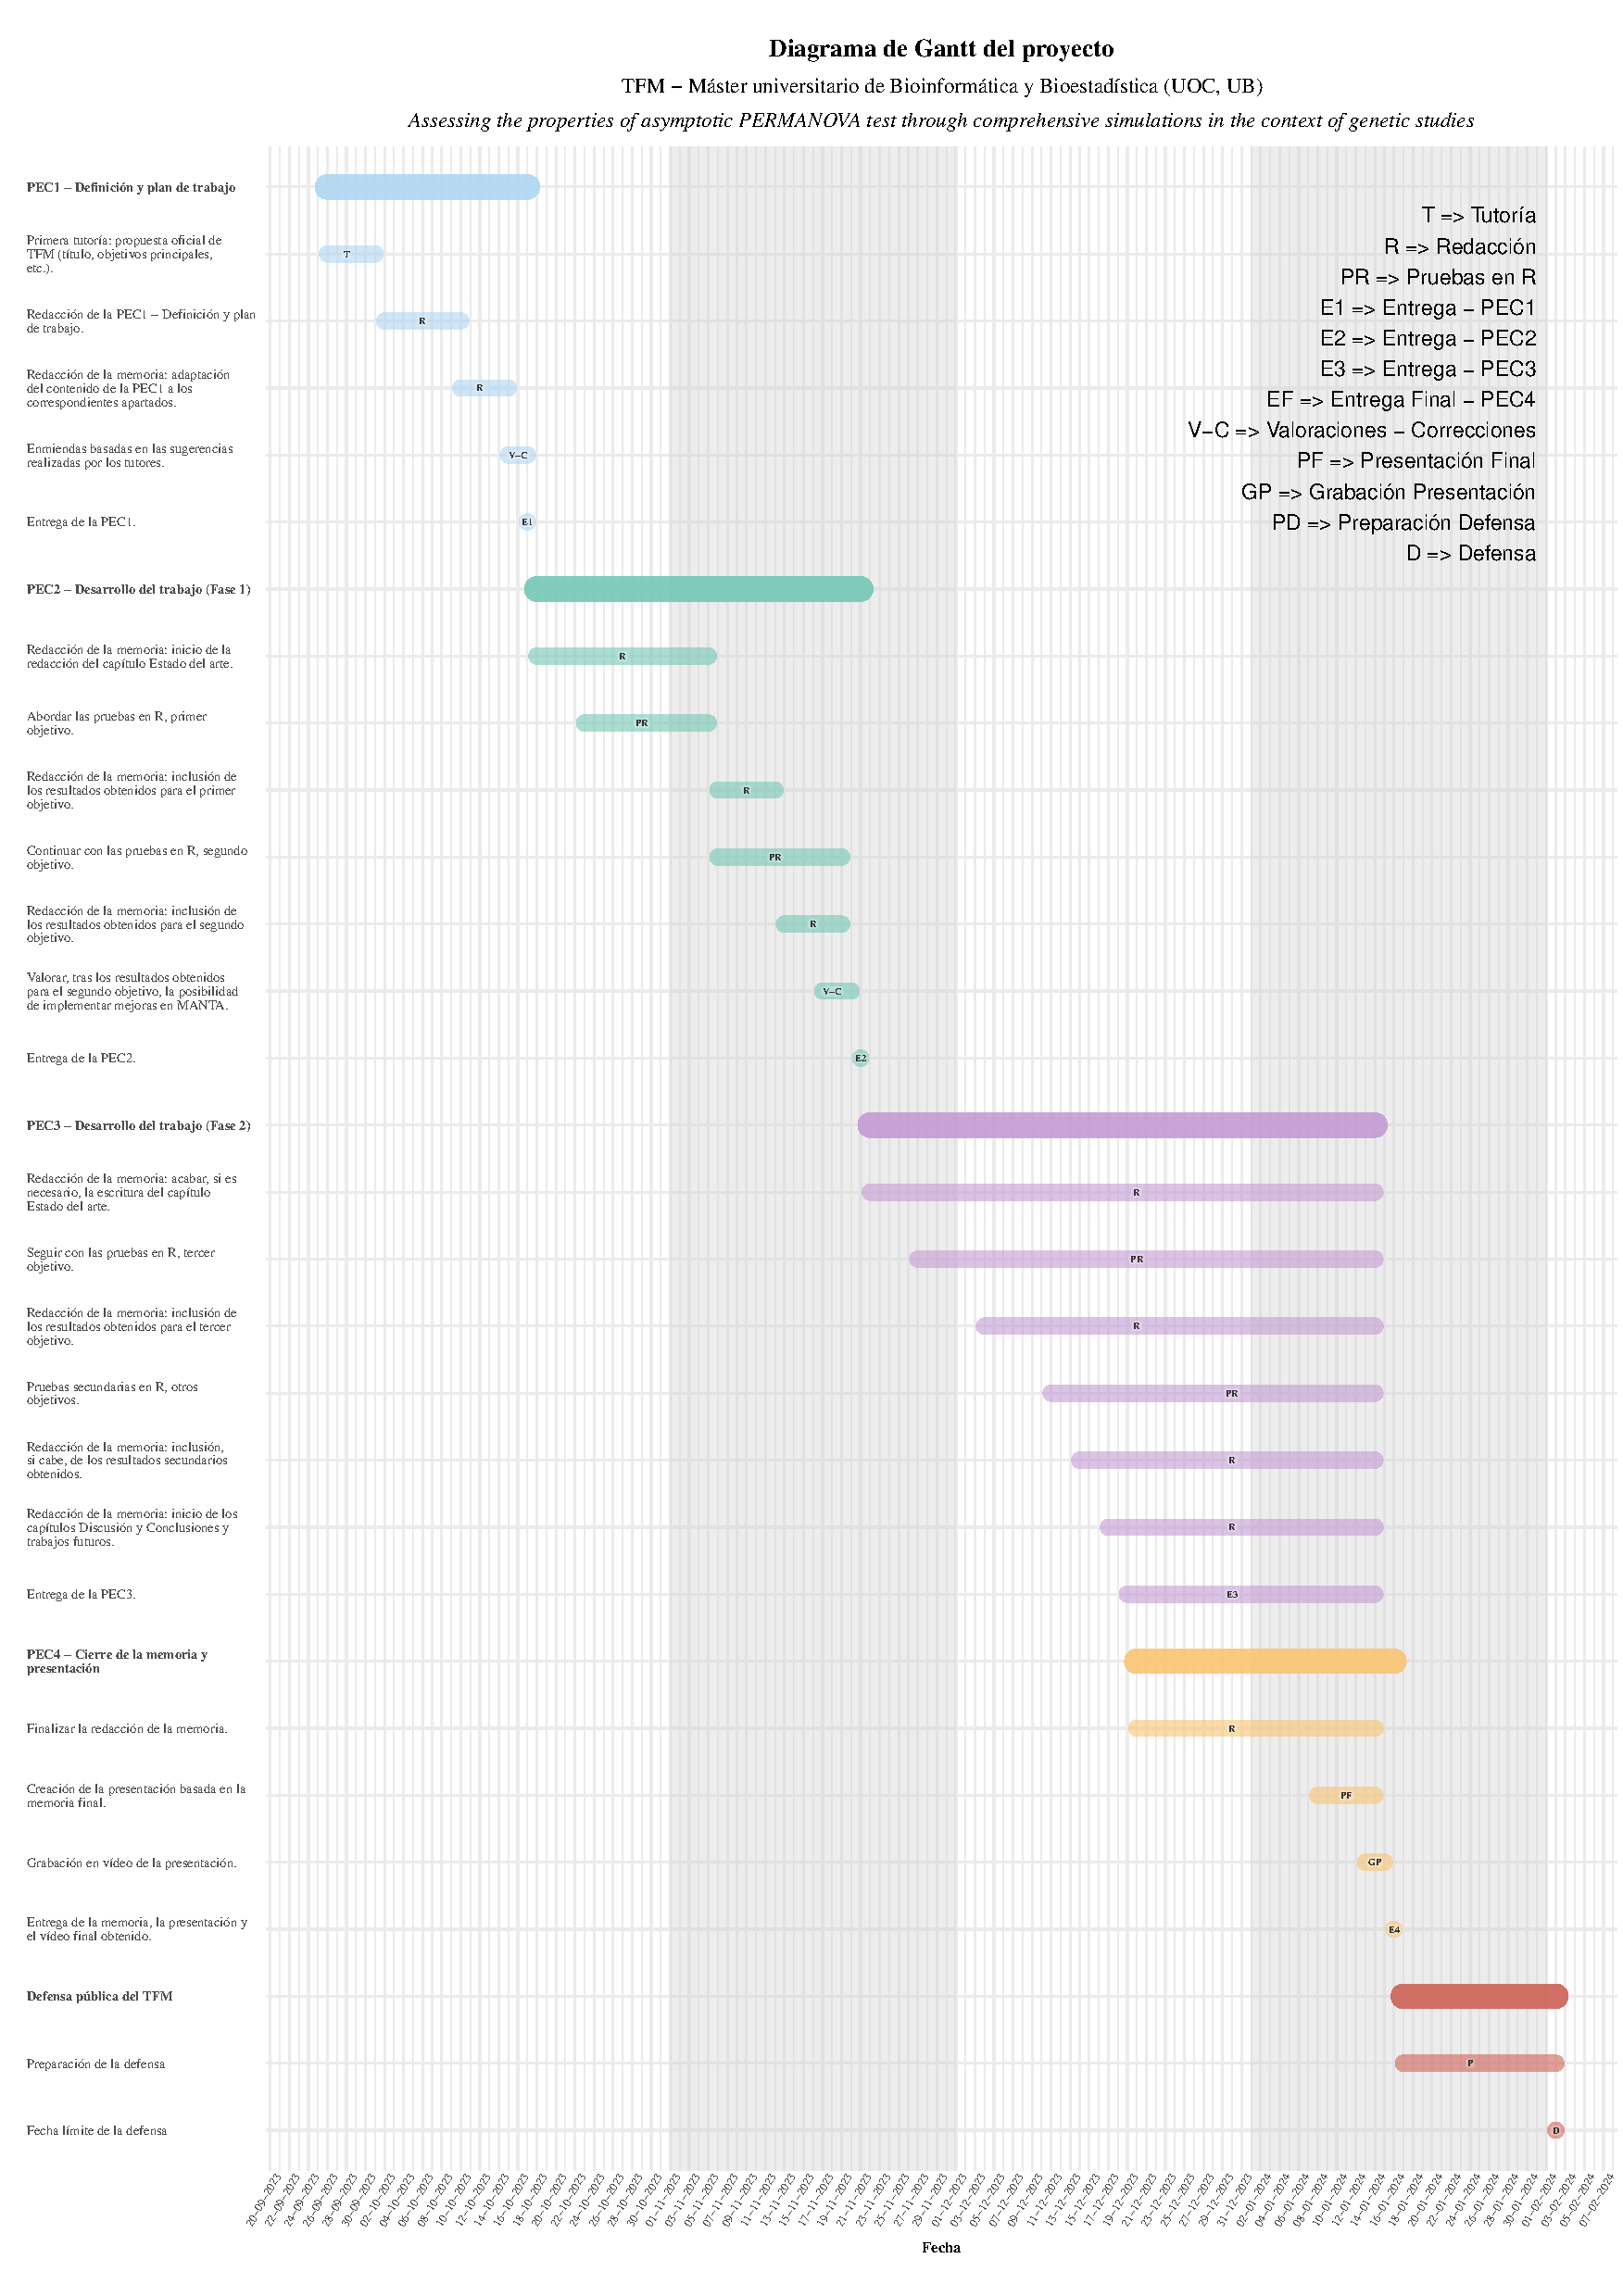
\includegraphics[scale=.45]{TFMGantt.pdf}
    \caption{\scriptsize{Planificación orientativa de las tareas a realizar para la consecución de la memoria y presentación del presente TFM: (\textit{supra}) desglose de los diferentes objetivos y tareas propuestas; (\textit{infra}) diagrama Gantt correspondiente.}}
    \label{fig:PEC1 - GANTT_TFM}
\end{figure}


\newpage
% \end{landscape}


\section{Hitos}
\label{sec:PEC1 - Hitos}

A continuación se muestran las distintas fases del proyecto según su compleción, indicando los posibles retrasos o problemas inesperados o no que, al surgir, pueden haber puesto en riesgo la consecución de las tareas previstas, y los objetivos establecidos:

\scriptsize

% Crear una lista con checkbox:
% Dentro del "todolist": \item, \item[\done] o \item[\wontfix] (Antiguos: \item[\cmark], \item[\xmark])

\begin{todolist}
  \item[\done] \textbf{Primera entrega:} \textit{PEC1 - Definición y plan de trabajo}
  \begin{todolist}
  \item[\done] Primera tutoría: propuesta oficial de TFM (título, objetivos principales, etc.).
  \item[\done] Redacción de la \textit{PEC1 - Definición y plan de trabajo}.
  \item[\done] Redacción de la memoria: adaptación del contenido de la \textit{PEC1} a los correspondientes apartados.
  \item[\done] Enmiendas basadas en las sugerencias realizadas por los tutores.
  \item[\done] Entrega de la \textit{PEC1}.
  \end{todolist}
\end{todolist}

\begin{todolist}
  \item \textbf{Segunda entrega:} \textit{PEC2 - Desarrollo del trabajo - Fase 1}
  \begin{todolist}
  \item Redacción de la memoria: inicio de la redacción del capítulo \textit{Estado del arte}.
  \item Abordar las pruebas en \textit{R}, primer objetivo: estudiar las propiedades de \textit{MANTA} en algunos escenarios comparando diferentes transformaciones de los datos.
  \item Redacción de la memoria: inclusión de los resultados obtenidos para el primer objetivo.
  \item Continuar con las pruebas en \textit{R}, segundo objetivo: estudiar la pérdida de potencia de la versión asintótica de \textit{PERMANOVA} con respecto a \textit{MANOVA} y otros métodos.
  \item Redacción de la memoria: inclusión de los resultados obtenidos para el segundo objetivo.
  \item Valorar, tras los resultados obtenidos para el segundo objetivo, la posibilidad de implementar mejoras en \textit{MANTA}.
  \item Entrega de la \textit{PEC2}.
  \end{todolist}
\end{todolist}

\begin{todolist}
  \item \textbf{Tercera entrega:} \textit{PEC3 - Desarrollo del trabajo - Fase 2}
  \begin{todolist}
  \item Redacción de la memoria: acabar, si es necesario, la escritura del capítulo \textit{Estado del arte}.
  \item Seguir con las pruebas en \textit{R}, tercer objetivo: comparar los resultados obtenidos con respecto al cálculo de la distribución de las formas cuadráticas entre el método \textit{Farebrother} (implementado para la versión asintótica de \textit{PERMANOVA} con \textit{MANTA}) y el de \textit{Saddlepoint}.
  \item Redacción de la memoria: inclusión de los resultados obtenidos para el tercer objetivo.
  \item Pruebas secundarias en \textit{R}, otros objetivos: extender el tercer objetivo, ampliando la comparativa \textit{Farebrother} vs. \textit{Saddlepoint} a otros métodos (\textit{Davies}, \textit{Imhof}, \textit{Liu}, etc.).
  \item Redacción de la memoria: inclusión, si cabe, de los resultados secundarios obtenidos.
  \item Redacción de la memoria: inicio de los capítulos \textit{Discusión} y \textit{Conclusiones y trabajos futuros}.
  \item Entrega de la \textit{PEC3}.
  \end{todolist}
\end{todolist}

\begin{todolist}
  \item \textbf{Cuarta entrega:} \textit{PEC4 - Cierre de la memoria y de la presentación}
  \begin{todolist}
  \item Finalizar la redacción de la memoria: adaptación del contenido generado en las diferentes \textit{PEC} a los correspondientes apartados, finalizando las secciones anexas (\textit{Bibliografía}, \textit{Glosario}, etc.).
  \item Creación, bajo los criterios establecidos, de la presentación basada en la memoria final.
  \item Grabación en vídeo de la presentación.
  \item Entrega de la memoria, la presentación y el vídeo final obtenido (sendas copias en el \textit{REC} y la aplicación \textit{Present@}).
  \end{todolist}
\end{todolist}

\begin{todolist}
  \item \textbf{Defensa:} \textit{Preparación para la defensa pública del TFM}
  \begin{todolist}
  \item Preparación de la defensa a la espera de la asignación definitiva de fecha.
  \item Defensa pública síncrona del TFM ante el tribunal asignado.
  \end{todolist}
\end{todolist}

\normalsize


\section{Análisis de riesgos}
\label{sec:PEC1 - Análisis de riesgos}

En esta sección se indicarán algunas de las contingencias que pudieran surgir durante la realización del proyecto, indicando, a su conclusión, si alguna de ellas ha impedido su apropiado avance o, incluso, la no consecución de alguno de los objetivos planteados:

\footnotesize

\begin{itemize}
\item \textit{\textbf{Tiempo limitado}:} debido a que el TFM debe realizarse en un solo cuatrimestre, el tiempo disponible para desarrollar el proyecto suele ser muy ajustado. Cualquier contratiempo o retraso en la planificación, ya sea predecible o no, puede afectar gravemente a la consecución de los plazos y, eventualmente, impedir alcanzar alguno de los objetivos que se han planteado. Ser capaz de maximizar la dedicación con el tiempo disponible, e identificar a tiempo los escollos que pueden atascar el proceso, serán claves para mitigar sus efectos.
\item \textit{\textbf{Planificación incorrecta}:} una posible mala priorización o asignación de tiempo a las tareas pertinentes puede influir de manera negativa en la consecución de los objetivos, sobre todo si existe dependencia de la tarea afectada por parte de alguna otra. También puede afectar de manera negativa una infravaloración de la dificultad de alguno de los objetivos propuestos, ya sea por el tiempo requerido para su consecución, o por falta de los conocimientos necesarios.
\item \textbf{Etapa de análisis y pruebas:} en ella pueden surgir diversos contratiempos, como la dificultad en el manejo de los \textit{scripts} de código que se pretenden utilizar, problemas inesperados con el computador utilizado, lentitud de los procesos ejecutados al tratar con grandes cantidades de datos, etc.
\end{itemize}

\normalsize


\section{Breve sumario de productos obtenidos}
\label{sec:PEC1 - Breve sumario de productos obtenidos}

\footnotesize

\begin{itemize}
    \item \textbf{Plan de trabajo:} documento donde se incluye una distribución de tareas según los objetivos determinados, puntos clave y tiempos necesarios (disponible en la sección \textit{\hyperref[sec:Planificación del trabajo]{Planificación del trabajo}}). Así mismo, también se incluye una valoración de los posibles riesgos que puedieran surgir a lo largo de la elaboración del proyecto.
    \item \textbf{Memoria:} producto derivado de todas las entregas parciales o \textit{PEC} (basado en la estructura recomendada por la UOC), donde se detallará el contexto científico, los resultados obtenidos según el procedimiento seguido y, finalmente, las conclusiones extraídas tras su interpretación.
    \item \textbf{Producto:} aun sin ser un objetivo principal, puede llegar a obtenerse una iteración mejorada del programario utilizado ya existente.
    \item \textbf{Presentación virtual del TFM:} exposición oral y visual basada en la memoria producida. En ella se resaltarán los aspectos más importantes del trabajo realizado, presentando las distintas fases del proyecto de forma resumida.
    \item \textbf{Autoevaluación del proyecto:} documento que, una vez finalizado el proyecto, debe redactarse para plasmar una evaluación crítica del trabajo realizado, determinando el grado de alcance de los objetivos, y valorando los aspectos potencialmente mejorables.
\end{itemize}

\normalsize


\newpage\null\thispagestyle{empty} % Página en blanco para separar la Memoria de las PEC

\Huge
\vfill

\textbf{Memoria}
\normalsize

\newpage



%%%%%%%%%%%%%%%%%%%
% Memoria del TFM %
%%%%%%%%%%%%%%%%%%%

%%%%%%%%%%%%%%%%%%%%%%%%%%%%%%%%%%%%%%%%%%
% Primera parte: Introducción  <--> PEC1 %
%%%%%%%%%%%%%%%%%%%%%%%%%%%%%%%%%%%%%%%%%%


\chapter{Introducción}
\label{chap:Introducción}


\section{Contexto y justificación del trabajo}
\label{sec:Contexto y justificación del trabajo}

% Contextualizad el TFM, explicad a qué ámbito pertenece, y justificad su interés: explicad por qué el trabajo que habéis elegido es interesante.


% Propuesta de TFM (D. Garrido y M. Calvo):
%
%  Título: Assessing the properties of asymptotic PERMANOVA test through comprehensive
%          simulations in the context of genetic studies
%
%  Objetivos principales:
%
%    - Estudio de potencia con distintas transformaciones (sqrt, log, datos composicionales, etc.)
%    - Estudio de la pérdida de potencia con respecto a MANOVA con P-valores pequeños
%    - Evaluación comparativa del método de Davies y el propuesto en Yang J. et al.
%      (implementación en C/C++)
%
%  Comentarios PEC1 (D. Garrido y M. Calvo):
%
%    - Acordarse que en todo caso trabajamos con la versión asintótica de PERMANOVA,
%                no con PERMANOVA!!! 
%
%    - Descripción más detallada:
%
%      a) GWAS y QTL mapping
%      b) Cómo en estos análisis se usan sobre todo métodos univariantes
%      c) Ventajas de las aproximaciones multivariantes
%      d) Limitaciones (parametricas, running time)
%      e) Cómo PERMANOVA puede ser una buena alternativa, pero necesita permutaciones,
%         razón por la que hemos desarrollado MANTA (= asymptotic PERMANOVA)
%      f) Aquí entra tu TFM: estudiar las propiedades de MANTA en algunos escenarios,
%         comparar transformaciones, estudiar pérdida de potencia vs MANOVA y otros métodos
%         (reportada en este artículo: https://www.nature.com/articles/s41588-022-01154-4), 
%         implementaciones (e.g. Farebrother -current- vs Saddlepoint), etc.
%         Nosotros ya hicimos benchmark Davies vs Farebrother vs Imhof vs Liu, aunque se puede ampliar,
%         el objetivo fundamental es comparar Farebrother con Saddlepoint.


El tema escogido para la realización del TFM se enmarca en el análisis de datos ómicos mediante el uso de la \hspace{-.5em}\textit{\gls{estadística multivariante}}, principalmente la versión asintótica de \hspace{-.5em}\textit{\gls{PERMANOVA}}, aplicada al estudio de asociaciones entre los polimorfismos de un solo nucleótido (\hspace{-.5em}\textit{\gls{SNPs}}) del genoma completo (estudios tipo \hspace{-.5em}\textit{\gls{GWAS}}) y algunos rasgos característicos, como son las principales enfermedades humanas, así como en la detección de \hspace{-.5em}\textit{\gls{sQTLs}} utilizando datos \hspace{-.5em}\textit{\gls{RNA-seq}}.

%      a) GWAS y QTL mapping
%      b) Cómo en estos análisis se usan sobre todo métodos univariantes

Originalmente, las investigaciones basadas en \textit{GWAS}, ya sea integrando \textit{sQTLs} o no, se han realizado con la finalidad de comprobar la asociación entre los \textit{SNPs} con diferentes variantes genéticas mediante el estudio de un único rasgo (única variable o \hspace{-.5em}\textit{\gls{trait}}), con lo que los análisis estadísticos correspondientes llevados a cabo suelen utilizar, lógicamente, los principales métodos univariantes disponibles (sumario estadístico basado en tablas de distribución de frecuencias, estadísticos de centralización o dispersión, etc.).

De este modo, este tipo de estudios, al centrarse en un solo \textit{trait} de todos los disponibles en el gran volumen de datos sobre fenotipos utilizable, no permiten tratar la posible relación causa-efecto subyacente, obteniendo un análisis meramente descriptivo. \\

%      c) Ventajas de las aproximaciones multivariantes
%      d) Limitaciones (parametricas, running time)
%      e) Cómo PERMANOVA puede ser una buena alternativa, pero necesita permutaciones,
%         razón por la que hemos desarrollado MANTA (= asymptotic PERMANOVA)

Alternativamente, gracias a la gran cantidad de datos disponibles últimamente con perfiles genómicos complejos (alta diversidad de rasgos moleculares), la necesidad de encontrar correlaciones entre las diferentes variables analizables y los rasgos de interés, ha resultado en un crecimiento en la utilización de métodos multivariantes para su análisis estadístico.

Las principales ventajas con respecto al enfoque univariante clásico, para poder determinar la posible estructura de correlaciones subyacente en los datos, pueden enumerarse como sigue:

{\small
\begin{itemize}
    \item Mayor potencia estadística para detectar asociaciones genéticas.
    \item Ofrece ventajas en el estudio de la \hspace{-.25em}\textit{\gls{pleiotropía}} (cuando el gen o alelo considerado es responsable de efectos fenotípicos o caracteres distintos y, a priori, no relacionados).
    \item Resulta de utilidad incluso cuando solo un pequeño grupo de los rasgos se ve afectado por el genotipo de interés.
    \item Permite el análisis a través de múltiples capas fenotípicas en bloque, dando luz sobre los mecanismos moleculares activados por las variantes genéticas consideradas.
    \item Posibilita la caracterización de los efectos genéticos sobre un mismo rasgo cuando este es medido en diferentes condiciones ambientales o entornos.
    \item Requiere de menos pruebas individuales, lo que disminuye las de carácter múltiple.
\end{itemize}}

Contrariamente, del uso de los métodos más habitualmente utilizados para estudiar estas asociaciones genéticas multirasgo emergen diversos inconvenientes, entre los cuales destacan:

{\small
\begin{itemize}
    \item Los métodos que modelan el genotipo como variable dependiente comprobando a su vez la asociación con una suma ponderada de fenotipos (\textit{MV-PLINK} (\cite{ferreira_multivariate_2009}) o análisis de correlación canónica, y \hspace{-.5em}\textit{\gls{MultiPhen}} \cite{coin_multiphen_2020} que utiliza la regresión ordinal) adolecen de la posibilidad de evaluar diseños complejos que presentan mutiples interacciones entre el genotipo y otras covariables.
    \item Tanto el análisis multivariante de la varianza (\hspace{-.5em}\textit{\gls{MANOVA}}), como el de los modelos multivariantes lineales mixtos (\hspace{-.5em}\textit{\gls{mvLMMs}}) \cite{zhou_efficient_2014}, resultan ser más tolerantes a estos diseños complejos al tratar los fenotipos como variables dependientes, introduciendo de froma natural el posible parentesco genético entre los individuos analizados. Esta ventaja se torna inconveniente para grandes conjuntos de datos, sobre todo para el método \textit{mvLMMs}, cuya continua mejora en su implementación computacional sigue requiriendo de tiempos excesivamente altos. 
    \item La pluralidad de los métodos de regresión multivariante presuponen una normalidad en la distribución de los errores del modelo que puede no llegar a cumplirse. Todo y que pueden aplicarse transformaciones individuales a cada rasgo estudiado, no puede garantizarse la normalidad multivariante, lo que resulta en una reducción de la potencia estadística en comparación con el modelo aplicado a los rasgos no transformados.
    \item Hasta el momento, las diversas implementaciones de \textit{métodos bayesianos} para el estudio de asociaciones multirasgo no han sido satisfactorias, requiriendo siempre un tiempo elevado de cálculo debido al coste computacional que implican.
    \item Para los métodos \hspace{-.5em}\textit{\gls{MTAR}} \cite{luo_multi-trait_2020} o \hspace{-.5em}\textit{\gls{MOSTest}} \cite{noauthor_precimedmostest_2023} \cite{van_der_meer_understanding_2020} existe la necesidad de garantizar la normalidad multivariante asintótica cuando se utilizan los sumarios estadísticos univariantes, lo que no es trivial, sumado a que evitar la aparición de sesgos en la estimación de correlaciones de rasgos a partir de esta clase de estadísticos no es sencillo (afectaciones de heredabilidad de los rasgos, patrones de desequilibrio de ligamiento, etc.).
\end{itemize}}

Con todo lo anterior, resulta evidente la necesidad de disponer de un método no paramétrico adecuado tanto para los estudios basados en (\textit{GWAS}) como en \textit{sQTLs}. El modelo de \textit{PERMANOVA} (\cite{anderson_new_2001}) amplía el modelo lineal factorial univariante a múltiples dimensiones sin requerir una distribución de probabilidad conocida de las variables dependientes, introduciendo un enfoque basado en la distancia, poniendo a prueba la hipótesis de ausencia de efectos mediante un procedimiento de permutación basado en un estadístico \hspace{-.5em}\textit{\gls{pseudo-F}}, en el que las sumas de cuadrados del \textit{ANOVA} se sustituyen por sumas de interdistancias entre observaciones.\\
Pese a ser exitoso en muchos estudios, dando buenos resultados en un tiempo de cálculo reducido para diseños fijos unidireccionales, resulta inviable en los estudios actuales, donde el mayor tamaño y complejidad de los conjuntos de datos requiere una precisión para el cálculo del valor p que este procedimiento permutacional no puede alcanzar en las condiciones requeridas.

El punto de partida del presente trabajo radica en los diversos estudios realizados con el fin de superar esta limitación. En concreto: sendos artículos de Garrido-Martín, D. \textit{et al.} (\cite{garrido-martin_fast_2022} y \cite{garrido-martin_identification_2021}), y el trabajo de Monlong, J. \textit{et al.} \cite{monlong_identification_2014}. Donde, gracias al programa \hspace{-.5em}\textit{\gls{MANTA}} (\cite{garrido-martin_manta_2023}, desarrollado principalmente en R), se estudia mediante diversas simulaciones (\cite{garrido-martin_manta-sim_2022}) de diseños complejos la distribución asintótica de la estadística de pruebas \textit{PERMANOVA} en el caso de la distancia euclídea (\hspace{-.5em}\textit{\gls{valores p}} de carácter no paramétrico y asintótico para modelos lineales multivariados), obteniendo resultados igualmente válidos tras cualquier transformación de los datos que preserve la independencia de las observaciones.

%      f) Aquí entra tu TFM: estudiar las propiedades de MANTA en algunos escenarios,
%         comparar transformaciones, estudiar pérdida de potencia vs MANOVA y otros métodos
%         (reportada en este artículo: https://www.nature.com/articles/s41588-022-01154-4), 
%         implementaciones (e.g. Farebrother -current- vs Saddlepoint), etc.
%         Nosotros ya hicimos benchmark Davies vs Farebrother vs Imhof vs Liu, aunque se puede ampliar,
%         el objetivo fundamental es comparar Farebrother con Saddlepoint.

La finalidad principal será ahondar en estos estudios, yendo más allá en al menos los siguientes aspectos:

{%\small
\begin{itemize}
    \item Estudiar las propiedades de \textit{MANTA} en algunos escenarios, determinando cómo los diferentes tipos de transformaciones de datos afectan a los resultados obtenidos, y dilucidar si existe algún protocolo privilegiado en las simulaciones implementadas.
    \item Estudiar la pérdida de potencia de la versión asintótica de \textit{PERMANOVA} con respecto a \textit{MANOVA} y otros métodos, profundizando en la afectación de la variación del nivel de significación considerado sobre la potencia de cada uno.
    \item Comparar los resultados obtenidos con respecto al cálculo de la distribución de las formas cuadráticas entre el método Farebrother (implementado para la versión asintótica de \textit{PERMANOVA} con \textit{MANTA}) y el de Saddlepoint.
    \item Extender el punto anterior, ampliando la comparativa Farebrother vs. Saddlepoint a otros métodos: métodos exactos como el de Davies, R. B. (\cite{davies_numerical_1973}, \cite{davies_algorithm_1980}), o aproximaciones numéricas como la de Liu–Tang–Zhang (\cite{qi_genetic_2022}), el método de Imhof, etc.
    \item Partiendo del caso de estudio anterior, y secundariamente, se llevaría a cabo la implementación del método más óptimo en el paquete \textit{MANTA} ya existente, en caso de que este exista.
\end{itemize}}

\text{ }

\section{Objetivos del trabajo}
\label{sec:Objetivos del trabajo}

% Explicad a grandes rasgos en qué consistirá el TFM. Este punto no debe confundirse con una introducción, sino que también debe explicar brevemente como planeáis que sea el trabajo.


%  Comentarios PEC1 (D. Garrido y M. Calvo):
%
%    - En este contexto yo no añadiría los objetivos como tal, describe un poco si quieres pero
%      ponlos en el apartado correspondiente
%    - Quizás puedes definir un objetivo general, que sea estudiar las propiedades de MANTA en
%      distintos contextos de simulación [...] y mejorar la implementación actual y luego añadir
%      los objetivos (que ahora llamas principales) como específicos. O alternativamente desarrollar
%      un par de objetivos específicos por cada uno de los principales.


De los diferentes puntos detallados en el apartado anterior, se extrae que el presente trabajo deberá permitirnos profundizar en aspectos concretos de los estudios ya referenciados (\cite{garrido-martin_fast_2022}, \cite{garrido-martin_identification_2021}), \cite{monlong_identification_2014}), con el objetivo último de determinar la validez de la versión asintótica del método \textit{PERMANOVA} (implementado en el paquete \textit{MANTA}) con respecto a otros métodos similares bajo un mismo conjunto de simulaciones computacionales complejas basadas en datos de escenarios reales.

\newpage

% Explicad claramente tanto los objetivos generales como los específicos:
% Objetivos generales: Deben ser pocos (quizás un par o máximo tres) y suficientemente amplios para cubrir todo el alcance del proyecto. Deben estar redactados de forma concreta y evaluable.
% Objetivos específicos: desglosad cada objetivo general en otros más concretos (no confundir con tareas). Se deben redactar con un verbo en infinitivo de significado medible (no puede ser por ejemplo “saber” porque no se puede medir  o evidenciar su cumplimiento).

Según las bases generales establecidas, y para una consecución satisfactoria del estudio propuesto, se han considerado los siguientes objetivos principales:

{\small
\begin{itemize}
    \item Estudiar las propiedades de \textit{MANTA} en algunos escenarios, determinando cómo los diferentes tipos de transformaciones de datos afectan a los resultados obtenidos, y dilucidar si existe algún protocolo privilegiado en las simulaciones implementadas.
    \item Estudiar la pérdida de potencia de la versión asintótica de \textit{PERMANOVA} con respecto a \textit{MANOVA} y otros métodos, profundizando en la afectación de la variación del nivel de significación considerado sobre la potencia de cada uno.
    \item Comparar los resultados obtenidos con respecto al cálculo de la distribución de las formas cuadráticas entre el método Farebrother (implementado para la versión asintótica de \textit{PERMANOVA} con \textit{MANTA}) y el de Saddlepoint.
\end{itemize}}

Como extensión de los mismos, resulta también conveniente establecer otros objetivos secundarios:

{\small
\begin{itemize}
    \item Extender el tercer objetivo principal, ampliando la comparativa Farebrother vs. Saddlepoint a otros métodos: métodos exactos como el de Davies, R. B. (\cite{davies_numerical_1973}, \cite{davies_algorithm_1980}), o aproximaciones numéricas como la de Liu–Tang–Zhang (\cite{qi_genetic_2022}), el método de Imhof, etc.
    \item Partiendo del caso de estudio anterior, se llevaría a cabo la implementación del método más óptimo en el paquete \textit{MANTA} ya existente, en caso de que los resultados obtenidos indiquen que alguno de ellos resulta ser más eficiente tanto computacional como estadísticamente hablando.
\end{itemize}}


% \section{Impacto en sostenibilidad, ético-social y de diversidad}
% \label{sec:Impacto en sostenibilidad, ético-social y de diversidad}
% 
% Esta sección tendría que identificar los impactos positivos y/o negativos del trabajo final en las tres dimensiones de la competencia transversal UOC “Compromiso ético y global”.
% 
% La Guía transversal sobre la Competencia Ética y Global os ayudará a redactar estos apartados.


\section{Enfoque y método seguido}
\label{sec:Enfoque y método seguido}

% Mención de cuáles son las posibles estrategias para llevar a cabo el trabajo y cuál es la estrategia elegida (desarrollar un producto nuevo, adaptar un producto existente...). Hay que incluir una valoración de por qué esta es la estrategia más apropiada para conseguir los objetivos.


% Indicad cuáles son las posibles estrategias para llevar a cabo el trabajo e indicar cuál es la elegida. Valorad por qué ésta es la más apropiada para lograr los objetivos.


%  Comentarios PEC1 (D. Garrido y M. Calvo):
%
%    - Desarrolla una lista de tareas y método a seguir, así como una planificación orientativa (Gannt).
%      Entiendo que serán preliminares, pero en cualquier caso estaría bien que te plantearas las
%      distintas tareas, así como que hicieras una pequeña evaluación de riesgos.

En cuanto al tiempo de dedicación, se ha enfocado el trabajo siguiendo las pautas marcadas por las diferentes entregas programadas por la UOC (\textit{Pruebas de Evaluación Continua} o \textit{PEC}), estableciendo los siguientes bloques de trabajo:

 % - Primera entrega: PEC1 - Definición y plan de trabajo
 %   * Primera tutoría: propuesta oficial de TFM (título, objetivos principales, etc.).
 %   * Redacción de la PEC1 - Definición y plan de trabajo.
 %   * Redacción de la memoria: adaptación del contenido de la PEC1 a los correspondientes apartados.
 %   * Enmiendas basadas en las sugerencias realizadas por los tutores.
 %   * Entrega de la PEC1.
 % 
 % - Segunda entrega: PEC2 - Desarrollo del trabajo - Fase 1
 %   * Redacción de la memoria: inicio de la redacción del capítulo Estado del arte.
 %   * Abordar las pruebas en R, primer objetivo: estudiar las propiedades de MANTA en algunos escenarios
 %   comparando diferentes transformaciones de los datos.
 %   * Redacción de la memoria: inclusión de los resultados obtenidos para el primer objetivo.
 %   * Continuar con las pruebas en R, segundo objetivo: estudiar la pérdida de potencia de la versión asintótica
 %   de PERMANOVA con respecto a MANOVA y otros métodos.
 %   * Redacción de la memoria: inclusión de los resultados obtenidos para el segundo objetivo.
 %   * Valorar, tras los resultados obtenidos para el segundo objetivo, la posibilidad de implementar mejoras en MANTA.
 %   * Entrega de la PEC2.
 % 
 % - Tercera entrega: PEC3 - Desarrollo del trabajo - Fase 2
 %   * Redacción de la memoria: acabar, si es necesario, la escritura del capítulo Estado del arte.
 %   * Seguir con las pruebas en R, tercer objetivo: comparar los resultados obtenidos con respecto al cálculo de la
 %   distribución de las formas cuadráticas entre el método Farebrother (implementado para la versión asintótica de
 %   PERMANOVA con MANTA y el de Saddlepoint.
 %   * Redacción de la memoria: inclusión de los resultados obtenidos para el tercer objetivo.
 %   * Pruebas secundarias en R, otros objetivos: extender el tercer objetivo, ampliando la comparativa Farebrother
 %   vs. Saddlepoint a otros métodos (Davies, Imhof, Liu, etc.).
 %   * Redacción de la memoria: inclusión, si cabe, de los resultados secundarios obtenidos.
 %   * Redacción de la memoria: inicio de los capítulos Discusión y Conclusiones y trabajos futuros.
 %   * Entrega de la PEC3.
 % 
 % - Cuarta entrega: PEC4 - Cierre de la memoria y de la presentación
 %   * Finalizar la redacción de la memoria: adaptación del contenido generado en las diferentes PEC  a los cor-
 %   respondientes apartados, finalizando las secciones anexas (Bibliografía, Glosario, etc.).
 %   * Creación, bajo los criterios establecidos, de la presentación basada en la memoria final.
 %   * Grabación en vídeo de la presentación.
 %   * Entrega de la memoria, la presentación y el vídeo final obtenido (sendas copias en el REC y la aplicación Present@).

\begin{itemize}
    \item \textbf{Primera entrega:} \textit{PEC1 - Definición y plan de trabajo} (5 \% de dedicación).
    \item \textbf{Segunda entrega:} \textit{PEC2 - Desarrollo del trabajo - Fase 1} (40 \% de dedicación).
    \item \textbf{Tercera entrega:} \textit{PEC3 - Desarrollo del trabajo - Fase 2} (40 \% de dedicación).
    \item \textbf{Cuarta entrega:} \textit{PEC4 - Cierre de la memoria y de la presentación} (10 \% de dedicación).
    \item \textbf{Defensa pública} (5 \% de dedicación).
\end{itemize}

Se puede encontrar una planificación más detallada en la sección \textit{\hyperref[sec:Planificación del trabajo]{Planificación del trabajo}}.


\newpage
% \begin{landscape}

\section{Planificación del trabajo}
\label{sec:Planificación del trabajo}

% Descripción de los recursos necesarios para hacer el trabajo, las tareas a realizar y una planificación temporal de cada tarea mediante un diagrama de Gantt o similar. Esta planificación tendría que marcar cuáles son los hitos parciales de cada una de las PEC.

% Desglosad las tareas que vais a hacer para conseguir vuestros objetivos y proponed una planificación temporal. 
% Tareas: Enumerad las diversas tareas en que se han desglosado los objetivos y la duración que se asigna a cada una. Tiene que haber una coherencia numérica entre objetivos generales, objetivos específicos y tareas.
% Calendario: Es recomendable usar un programa específico de planificación para generar un diagrama de Gantt que se pueda insertar en el documento.
% Hitos: Los hitos marcan los estados intermedios del proyecto y permiten avanzar en sucesivas etapas de resultados prácticos, por ejemplo, tomando decisiones relevantes. Es imprescindible que seáis estrictos en el cumplimiento de las fechas que os marquéis. Será importante que os baséis en el Plan Docente y concretamente en las fechas clave que se indican allá para elaborar vuestra planificación.
% Análisis de riesgos: Enumerad y comentad qué factores pueden repercutir negativamente en el seguimiento del plan de trabajo y en la consecución del proyecto. Hay dos factores que tienen influencia en cualquier proyecto: el alcance del proyecto  y el tiempo del que disponéis para realizarlo. Hay otros riesgos asociados a las características específicas de cada TFM y al método de investigación y/o de desarrollo que se utiliza. Igual que los objetivos, deben ser concretos. 

Una planificación orientativa de las tareas que conforman cada bloque de trabajo específico ideado, basados en la estructura de las diferentes PEC a entregar y de las necesidades del tema escogido, puede encontrarse en \ref{fig:PEC1 - GANTT_TFM}. 

% \footnote{Esta página se muestra de forma apaisada deliberadamente, con tal de acomodar la imagen correctamente.}

\begin{figure}[!htbp]
    \centering
    % \includegraphics[width=22truecm]{GANTT_TFM.png}
    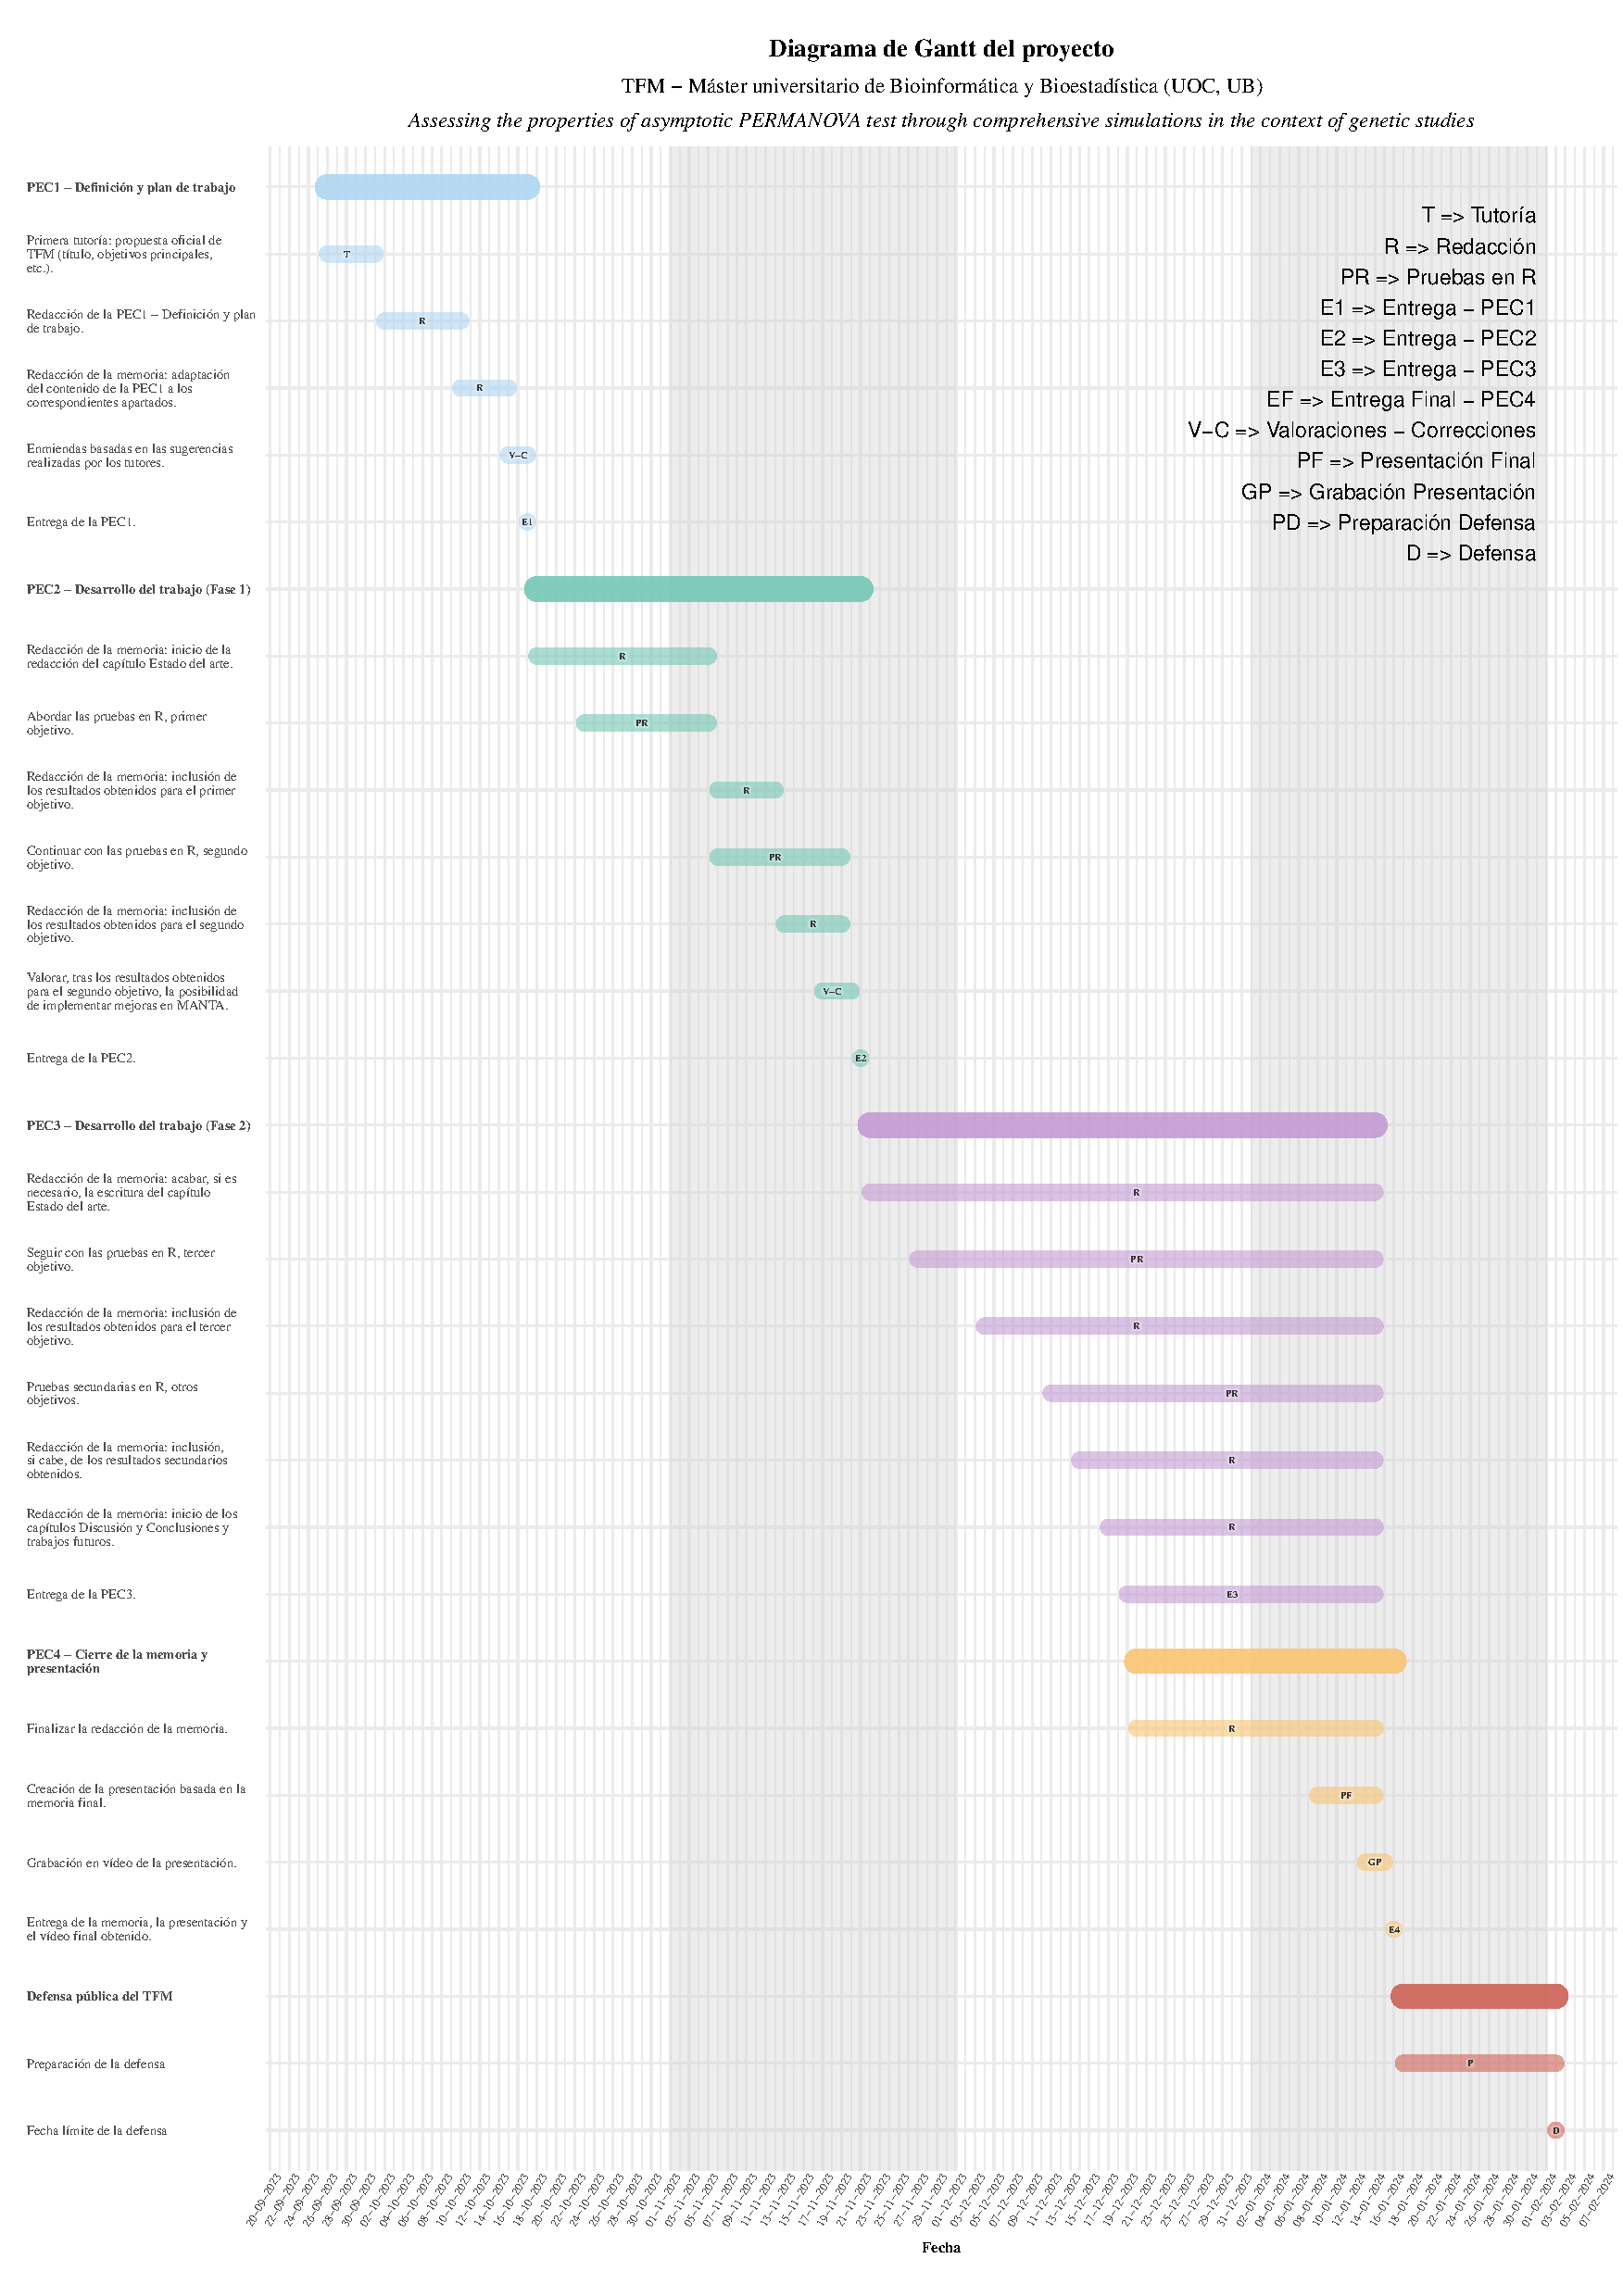
\includegraphics[scale=.45]{TFMGantt.pdf}
    \caption{\scriptsize{Planificación orientativa de las tareas a realizar para la consecución de la memoria y presentación del presente TFM: (\textit{supra}) desglose de los diferentes objetivos y tareas propuestas; (\textit{infra}) diagrama Gantt correspondiente.}}
    \label{fig:GANTT_TFM}
\end{figure}


\newpage
% \end{landscape}


\section{Hitos}
\label{sec:Hitos}

A continuación se muestran las distintas fases del proyecto según su compleción, indicando los posibles retrasos o problemas inesperados o no que, al surgir, pueden haber puesto en riesgo la consecución de las tareas previstas, y los objetivos establecidos:

\scriptsize

% Crear una lista con checkbox:
% Dentro del "todolist": \item, \item[\done] o \item[\wontfix] (Antiguos: \item[\cmark], \item[\xmark])

\begin{todolist}
  \item[\done] \textbf{Primera entrega:} \textit{PEC1 - Definición y plan de trabajo}
  \begin{todolist}
  \item[\done] Primera tutoría: propuesta oficial de TFM (título, objetivos principales, etc.).
  \item[\done] Redacción de la \textit{PEC1 - Definición y plan de trabajo}.
  \item[\done] Redacción de la memoria: adaptación del contenido de la \textit{PEC1} a los correspondientes apartados.
  \item[\done] Enmiendas basadas en las sugerencias realizadas por los tutores.
  \item[\done] Entrega de la \textit{PEC1}.
  \end{todolist}
\end{todolist}

\begin{todolist}
  \item \textbf{Segunda entrega:} \textit{PEC2 - Desarrollo del trabajo - Fase 1}
  \begin{todolist}
  \item Redacción de la memoria: inicio de la redacción del capítulo \textit{Estado del arte}.
  \item Abordar las pruebas en \textit{R}, primer objetivo: estudiar las propiedades de \textit{MANTA} en algunos escenarios comparando diferentes transformaciones de los datos.
  \item Redacción de la memoria: inclusión de los resultados obtenidos para el primer objetivo.
  \item Continuar con las pruebas en \textit{R}, segundo objetivo: estudiar la pérdida de potencia de la versión asintótica de \textit{PERMANOVA} con respecto a \textit{MANOVA} y otros métodos.
  \item Redacción de la memoria: inclusión de los resultados obtenidos para el segundo objetivo.
  \item Valorar, tras los resultados obtenidos para el segundo objetivo, la posibilidad de implementar mejoras en \textit{MANTA}.
  \item Entrega de la \textit{PEC2}.
  \end{todolist}
\end{todolist}

\begin{todolist}
  \item \textbf{Tercera entrega:} \textit{PEC3 - Desarrollo del trabajo - Fase 2}
  \begin{todolist}
  \item Redacción de la memoria: acabar, si es necesario, la escritura del capítulo \textit{Estado del arte}.
  \item Seguir con las pruebas en \textit{R}, tercer objetivo: comparar los resultados obtenidos con respecto al cálculo de la distribución de las formas cuadráticas entre el método \textit{Farebrother} (implementado para la versión asintótica de \textit{PERMANOVA} con \textit{MANTA}) y el de \textit{Saddlepoint}.
  \item Redacción de la memoria: inclusión de los resultados obtenidos para el tercer objetivo.
  \item Pruebas secundarias en \textit{R}, otros objetivos: extender el tercer objetivo, ampliando la comparativa \textit{Farebrother} vs. \textit{Saddlepoint} a otros métodos (\textit{Davies}, \textit{Imhof}, \textit{Liu}, etc.).
  \item Redacción de la memoria: inclusión, si cabe, de los resultados secundarios obtenidos.
  \item Redacción de la memoria: inicio de los capítulos \textit{Discusión} y \textit{Conclusiones y trabajos futuros}.
  \item Entrega de la \textit{PEC3}.
  \end{todolist}
\end{todolist}

\begin{todolist}
  \item \textbf{Cuarta entrega:} \textit{PEC4 - Cierre de la memoria y de la presentación}
  \begin{todolist}
  \item Finalizar la redacción de la memoria: adaptación del contenido generado en las diferentes \textit{PEC} a los correspondientes apartados, finalizando las secciones anexas (\textit{Bibliografía}, \textit{Glosario}, etc.).
  \item Creación, bajo los criterios establecidos, de la presentación basada en la memoria final.
  \item Grabación en vídeo de la presentación.
  \item Entrega de la memoria, la presentación y el vídeo final obtenido (sendas copias en el \textit{REC} y la aplicación \textit{Present@}).
  \end{todolist}
\end{todolist}

\begin{todolist}
  \item \textbf{Defensa:} \textit{Preparación para la defensa pública del TFM}
  \begin{todolist}
  \item Preparación de la defensa a la espera de la asignación definitiva de fecha.
  \item Defensa pública síncrona del TFM ante el tribunal asignado.
  \end{todolist}
\end{todolist}

\normalsize


\section{Análisis de riesgos}
\label{sec:Análisis de riesgos}

En esta sección se indicarán algunas de las contingencias que pudieran surgir durante la realización del proyecto, indicando, a su conclusión, si alguna de ellas ha impedido su apropiado avance o, incluso, la no consecución de alguno de los objetivos planteados:

\footnotesize

\begin{itemize}
\item \textit{\textbf{Tiempo limitado}:} debido a que el TFM debe realizarse en un solo cuatrimestre, el tiempo disponible para desarrollar el proyecto suele ser muy ajustado. Cualquier contratiempo o retraso en la planificación, ya sea predecible o no, puede afectar gravemente a la consecución de los plazos y, eventualmente, impedir alcanzar alguno de los objetivos que se han planteado. Ser capaz de maximizar la dedicación con el tiempo disponible, e identificar a tiempo los escollos que pueden atascar el proceso, serán claves para mitigar sus efectos.
\item \textit{\textbf{Planificación incorrecta}:} una posible mala priorización o asignación de tiempo a las tareas pertinentes puede influir de manera negativa en la consecución de los objetivos, sobre todo si existe dependencia de la tarea afectada por parte de alguna otra. También puede afectar de manera negativa una infravaloración de la dificultad de alguno de los objetivos propuestos, ya sea por el tiempo requerido para su consecución, o por falta de los conocimientos necesarios.
\item \textbf{Etapa de análisis y pruebas:} en ella pueden surgir diversos contratiempos, como la dificultad en el manejo de los \textit{scripts} de código que se pretenden utilizar, problemas inesperados con el computador utilizado, lentitud de los procesos ejecutados al tratar con grandes cantidades de datos, etc.
\end{itemize}

\normalsize


\section{Breve sumario de productos obtenidos}
\label{sec:Breve sumario de productos obtenidos}

% No hay que entrar en detalle: la descripción detallada se hará en el resto de capítulos.

% En este apartado debéis concretar qué se obtendrá al final del proyecto. Tienen que ser ítems tangibles y medibles de lo que se espera obtener. Recordad que estos resultados deberán incluir los entregables que os pedimos al final del trabajo:
% Plan de trabajo.
% Memoria.
% Producto, si es que hay un producto resultado que no se incluye en la memoria, por ejemplo un artículo, un software desarrollado, etc.
% Presentación virtual.

\footnotesize

\begin{itemize}
    \item \textbf{Plan de trabajo:} documento donde se incluye una distribución de tareas según los objetivos determinados, puntos clave y tiempos necesarios (disponible en la sección \textit{\hyperref[sec:Planificación del trabajo]{Planificación del trabajo}}). Así mismo, también se incluye una valoración de los posibles riesgos que puedieran surgir a lo largo de la elaboración del proyecto.
    \item \textbf{Memoria:} producto derivado de todas las entregas parciales o \textit{PEC} (basado en la estructura recomendada por la UOC), donde se detallará el contexto científico, los resultados obtenidos según el procedimiento seguido y, finalmente, las conclusiones extraídas tras su interpretación.
    \item \textbf{Producto:} aun sin ser un objetivo principal, puede llegar a obtenerse una iteración mejorada del programario utilizado ya existente.
    \item \textbf{Presentación virtual del TFM:} exposición oral y visual basada en la memoria producida. En ella se resaltarán los aspectos más importantes del trabajo realizado, presentando las distintas fases del proyecto de forma resumida.
    \item \textbf{Autoevaluación del proyecto:} documento que, una vez finalizado el proyecto, debe redactarse para plasmar una evaluación crítica del trabajo realizado, determinando el grado de alcance de los objetivos, y valorando los aspectos potencialmente mejorables.
\end{itemize}

\normalsize


\section{Descripción de otros capítulos}
\label{sec:Descripción de otros capítulos}

En esta sección se realizará, en caso de ser necesario, una escueta descripción de los diversos capítulos de la memoria.

% Breve explicación de los contenidos de cada capítulo y su relación con el proyecto global.


%  ========================================>    GLOSARIO DE LA PRIMERA PARTE HECHO A DÍA 9/5/23    <==========================================  %
%  ========================================> PRIMERA PARTE CORREGIDA ORTOGRÁFICAMENTE A DÍA 9/5/23 <==========================================  %


%%%%%%%%%%%%%%%%%%%%%%%%%%%%%%%%%%%%%%%%%%%%%%%%%%%%%%%%%%%%%%%%%%%
% Segunda parte: Estado del arte + Primeros resultados  <--> PEC2 %
%%%%%%%%%%%%%%%%%%%%%%%%%%%%%%%%%%%%%%%%%%%%%%%%%%%%%%%%%%%%%%%%%%%


\chapter{Estado del arte}
\label{chap:Introducción}

% Estado del arte del tema en cuestión.
% Tendría que acabar mostrando por qué el trabajo es importante y que aporta algo, y con las hipótesis del trabajo.
% 
% 
% En estos apartados, hay que describir:
% \begin{itemize}
%     \item Los aspectos más relevante del diseño y desarrollo del trabajo.
%     \item La metodología elegida para hacer este desarrollo, describiendo las alternativas posibles, las decisiones tomadas, y los criterios utilizados para tomar estas decisiones.
%     \item Los productos obtenidos.
% \end{itemize}

...

% \section{Contexto biotecnológico}
% \label{sec:Contexto biotecnológico}
% 
% Aunque el presente trabajo es eminentemente teórico, centrándose en una comparativa de métodos estadísticos multivariantes específicos, aplicables a diversos campos de investigación, cabe destacar su aplicación biológica, en concreto, en la investigación genética avanzada.
% 
% Esta ha evolucionado enormemente en las últimas décadas gracias al desarrollo de nuevas tecnologías, permitiendo identificar variantes genéticas asociadas a una amplia variedad de fenotipos y rasgos. La secuenciación de nucleótidos que conforman la molécula de \textit{ADN} permite el análisis detallado de su estructura, convirtiéndose en la herramienta idonea para identificar variantes en el material genético.
% 
% En los años 70, la \textit{secuenciación Sanger} revolucionó la investigación originando la era genómica, la cual se ha asentado gracias a la evolución que ha sufrido este campo en los últimos años debido al desarrollo de las nuevas plataformas de secuenciación de alto rendimiento (\textit{Next-Generation Sequencing} o \textit{NGS}). Estas nuevas técnicas son capaces de generar paralelamente, y de forma masiva, millones de fragmentos de \textit{ADN} en un único proceso de secuenciación, consiguiendo así el análisis de grandes cantidades de información genética en una escala inimaginable en los orígenes de esta disciplina \cite{behjati_what_2013,noauthor_next-generation_nodate}.
% 
% Recientemente, cada vez más investigaciones han empezado a decantarse por un tipo específico de secuenciación masiva: la \textit{secuenciación de ARN} o \textit{RNA-seq}. Dicha estrategia de análisis utiliza técnicas \textit{NGS} para revelar la presencia y cantidad de \textit{ARN} existente en una muestra biológica en un momento dado, lo cual le permite ser aplicada para analizar cambios en el transcriptoma. Algunos usos potenciales de esta técnica que cabe destacar son \cite{wang_rna-seq_2009} \cite{noauthor_rna-seq_2023}:
% 
% \footnotesize
% 
% \begin{itemize}
%     \item Observación de transcritos resultantes del \textit{empalme alternativo}, \textit{modificación postranscripcional}, \textit{fusiones génicas}, \textit{mutaciones/polimorfismos de nucleótidos únicos} o \textit{SNP} y \textit{cambios de expresión de genes}.
%     \item Caracterización de diferentes poblaciones de \textit{ARN}: \textit{miARN}, \textit{tARN}, y \textit{rARN}.
%     \item Determinación de las \textit{fronteras exón/intrón}
%     \item Verificación y corrección de \textit{regiones 5' y 3'}.
% \end{itemize}
% 
% \normalsize
% 
% Pese a que la \textit{RNA-seq} es similar a la \textit{secuenciación de ADN}, existe una importante diferencia. En esta, se añade un paso más, de forma que en vez de aislar directamente el \textit{ADN}, se extrae primero el \textit{ARN} de la muestra transcribiéndolo seguidamente al revés para producir \textit{cDNA}, el cual se fragmenta y procesa mediante un sistema \textit{NGS} de alto rendimiento. Cabe añadir que la alta reproducibilidad de esta tecnologia y la reducción en la duración de todo el proceso, ya situado en menos de 24 horas (incluyendo el tiempo de preparación de la biblioteca, la secuenciación en sí, y el análisis bioinformático), la convierte en una de las estrategias de análisi genético más accesible y utilizada.
% 
% Gracias a estas técnicas de secuenciación masiva, los estudios de asociación del genoma completo (\textit{GWAS}) han sido hasta ahora el enfoque prioritario en cuanto a los esfuerzos por identificar variantes genéticas asociadas con un fenotipo o rasgo particular. Esta estrategia analiza la variación genética en todo el genoma de un gran número de individuos para identificar regiones asociadas con el rasgo de interés, resultando especialmente útil en la identificación de variantes genéticas asociadas con enfermedades comunes y complejas, así como con rasgos específicos. En concreto, este tipo de estudios destacan por su eficiencia en los siguientes campos \cite{tam_benefits_2019, garrido_martin_multivariate_2020, qi_genetic_2022, turner_quality_2011, noauthor_genome-wide_2023}:
% 
% \footnotesize
% 
% \begin{itemize}
%     \item En la identificación de nuevas \textit{asociaciones variante-rasgo}, estableciendo con éxito \textit{loci} de riesgo para un gran número de enfermedades y rasgos. Aunque no pueden explicar toda la heredabilidad de los rasgos complejos, representan un medio práctico por el cual se pueden descubrir asociaciones genuinas. De forma que con el aumento del número de muestras \textit{GWAS} se deberían seguir determinando nuevos \textit{loci}.
%     \item Los \textit{GWAS} pueden conducir al descubrimiento de nuevos mecanismos biológicos. Los \textit{loci GWAS} suelen implicar genes de función desconocida o que no se consideraban relevantes, cuyo seguimiento experimental puede conducir al descubrimiento de nuevos mecanismos biológicos subyacentes a las enfermedades.
%     \item Tiene diversas aplicaciones clínicas, ya que las variantes genéticas descubiertas mediante \textit{GWAS} pueden utilizarse para identificar a individuos con alto riesgo de padecer determinadas enfermedades, mejorando así la evolución de los pacientes mediante la detección precoz, la prevención o el tratamiento. Sus hallazgos pueden aplicarse a la clasificación y subtipificación de enfermedades.
%     \item Pueden aportar información sobre la etnicidad de ciertos rasgos complejos, ya que se conoce que algunos \textit{loci} de riesgo muestran considerables diferencias étnicas en frecuencia y/o tamaño del efecto.
%     \item También son relevantes para el estudio de variantes raras y de baja frecuencia. En la actualidad, la mayor parte de este tipo de estudios se realizan utilizando datos obtenidos mediante \textit{arrays de SNP} que, al incluir actualmente una mayor densidad de variantes y una gama más amplia de frecuencias alélicas, permiten genotipar directamente muchas variantes raras y de baja frecuencia. Las variantes raras y de baja frecuencia también pueden genotiparse utilizando matrices personalizadas centradas en exomas.
%     \item Otras aplicaciones son: puede utilizarse para \textit{identificar nuevos genes de enfermedades monogénicas y oligogénicas}, puede \textit{estudiar variantes genéticas distintas de los SNV}, sus datos se utilizan para \textit{múltiples aplicaciones más allá de la identificación de genes}, además, la \textit{generación, gestión y análisis de datos GWAS son sencillos}, además, al ser fácilmente compartibles y de acceso público, \textit{facilitan nuevos descubrimientos}.
% \end{itemize}
% 
% \normalsize
% 
% Cabe destacar uno de estos puntos, ya que representa a la mayoría de los estudios tipo \textit{GWAS} que se realizan hoy en día. Es el caso de las investigaciones que utilizan datos \textit{GWAS basados en arrays de SNP}, que ofrecen unas ventajas particulares:
% 
% \footnotesize
% 
% \begin{itemize}
%     \item \textbf{Utilizan una tecnología de \textit{genotipado} muy precisa}: lo que es crucial para el éxito de cualquier estudio de asociación genética a gran escala, donde los sesgos sistemáticos inducidos por las fuentes de error (aunque sean pequeñas) pueden hacer crecer tanto los falsos positivos como negativos a la hora de determinar las \textit{asociaciones variante-rasgo}. Concretamente, en la actualidad las \textit{matrices SNP} de genoma completo contemporáneas alcanzan precisiones por encima del 99,7 \% y, además, se han desarrollado protocolos que detrminan la utilización de solo aquellos datos que superen los umbrales de calidad para cada uno de los indicadores (\textit{call rate}, concordancia de duplicados, consistencia mendeliana y prueba de equilibrio de Hardy-Weinberg), establecidos de forma independiente para cada estudio, garantizando así la confianza en los resultados.
%     \item \textbf{Rentabilidad (coste y tiempo) a la hora de identificar \textit{loci de riesgo}}: es un método rentable ya que el coste del análisis de \textit{matrices SNP} seguido de la \textit{imputación de variantes hasta un MAF del 0,1 \%} se ha ido reduciendo durante los últimos años de forma constante. Este hecho permite, hoy en día, explorar gran parte de la variación genética del genoma a un coste razonable incluso en muestras de gran tamaño.
% \end{itemize}
% 
% \normalsize
% 
% Por otro lado, también presentan algunas limitaciones, entre las cuales se destacan las siguientes \cite{tam_benefits_2019, turner_quality_2011, noauthor_genome-wide_2023}:
% 
% \footnotesize
% 
% \begin{itemize}
%     \item Estos estudios se ven altamente afectados por la necesidad de adoptar un alto nivel de significación para tener en cuenta las pruebas múltiples realizadas, lo que comúnmente se realiza usando una \textit{corrección de Bonferroni} para mantener la tasa de falsos positivos en todo el genoma en un 5 \% (basado en la suposición de \num{1e6} pruebas independientes para la variación genética común). Todo esto afecta a la \textit{potencia} de esta técnica para detectar toda la hereditariedad explicada por los \textit{SNPs}, ya que las señales de asociación deberán alcanzar un umbral de \textbf{P}<\num{5e-8} para ser consideradas significativas. \\
% Una estrategia útil en algunas ocasiones para superar esta limitación es aumentar el tamaño de la muestra; en otras ocasiones, reducir el número de pruebas realizadas (lo cual se logra utilizando pruebas de asociación basadas en genes o limitando los análisis a regiones genómicas candidatas) es lo más adecuado.
%     \item Pese a haber identificado un número sin precedentes de variantes genéticas asociadas con enfermedades y rasgos comunes, sólo es capaz de explicar una pequeña parte de la heredabilidad estimada de los rasgos más complejos. Una probable explicación es que los \textit{SNPs} que afectan moderadamente se pierden porque no alcanzan el estricto umbral de significación establecido. El aumento constante en los tamaños de muestras, así como la adopción de nuevos métodos y diseños de estudio, pueden ayudar a solventar dicho escollo.
%     \item La correlación local de múltiples variantes genéticas debido al desequilibrio de enlace facilita la identificación inicial de un \textit{locus} pero dificulta el discernimiento de la variante o variantes causales. Una vez que se ha realizado un \textit{GWAS}, a menudo se requieren pasos adicionales para identificar las variantes causales y sus genes de destino. Los avances en los métodos estadísticos como los enfoques bayesianos, han permitido avanzar en la restricción de las posibles variantes causales. \\
%     Además, el aumento de bases de datos de elementos reguladores en una variedad de tipos de tejidos y células, disponibles públicamente  (ENCODE, Epigenome RoadMap, FANTOM5 y GTEx), así como herramientas para la consulta de dichos bancos de datos, ha permitido integrar los hallazgos de \textit{GWAS} con datos de genómica funcional en múltiples niveles, priorizando las variantes candidatas para el seguimiento funcional.
%     \item Otras limitaciones también son: que no se pueden identificar todos los determinantes genéticos de rasgos complejos; su poca fiabilidad en la detección de epistasis en humanos; que las señales analizadas pueden deberse a la estratificación criptica de la población; usualmente, tienen una capacidad predictiva clínicoa limitada.
%     \item En cuanto a los \textit{GWAS basados en arrays de SNP}, existen algunas limitaciones particulares:
%     \begin{itemize}
%         \item Dependen de la integridad de los estudios de secuenciación y los paneles de referencia resultantes que se utilizan para informar al diseño de matriz de genotipado e imputar variantes no tipadas en \textit{GWAS}. Las primeras configuraciones de SNP para todo el genoma fueron diseñados seleccionando \textit{SNPs} de los paneles de referencia de poblaciones predominantemente europeas, generando así un sesgo, y eludiendo la influencia que la variación de los patrones de desequilibrio de enlace entre grupos étnicos pueda tener. De un tiempo a esta parte, se ha intentado solventar desarrollando una nueva generación de matrices de alta densidad cuyos contenidos se basan en datos de secuenciación de poblaciones más diversas. Sin embargo, muchos grupos étnicos todavía no han sido secuenciados.
%         \item Aunque la evidencia empírica sugiere que gran parte de la heredabilidad de los rasgos complejos puede explicarse por variantes comunes, también se considera que las variantes raras y ultra raras han de contribuir de alguna manera. En este contexto, es destacable el hecho que hoy en día los \textit{GWAS basados en arrays de SNP} son incapaces de detectar variantes ultrararas asociadas con la enfermedad.
%     \end{itemize}
% \end{itemize}
% 
% \normalsize
% 
% 
% Por otro lado, en este tipo de estudios una proporción de las variantes descritas son \textit{QTLs} (\textit{eQTLs}, \textit{trQTLs}, etc.), siendo de particular interés los \textit{locus de rasgo cuantitativo de empalme} (\textit{sQTLs}), los cuales regulan el empalme alternativo del \textit{pre-ARNm}, y pueden ser detectados usando datos \textit{RNA-seq} \cite{noauthor_splicing_2021, monlong_identification_2014}. De esta manera, la correcta integración del genoma secuenciado, los \textit{QTLs} y el fenotipo celular, puede ayuda a comprender los genes causantes de ciertas enfermedades, las variantes genéticas causales que subyacen a los \textit{GWAS} y los procesos biológicos que intervienen.
% 
% Un \textit{locus de rasgo cuantitativo} (\textit{QTL}) es una sección de ADN que se correlaciona con la variación de un rasgo cuantitativo en el fenotipo de una población de organismos. Estos pueden mapearse de manera que permitan identificar qué marcadores moleculares, \textit{SNPs} o \textit{Polimorfismos en la longitud de fragmentos amplificados} (\textit{AFLPs}), se correlacionan con un rasgo observado, lo que suele ser un primer paso en la secuenciación e identificación de los genes que realmente modulan la expresión génica. \\
% Este mapeo permite descubrir regiones genómicas asociadas a la regulación de la transcripción de genes que pueden relacionarse con la variación fenotípica cuando se colocan con \textit{QTLs} (efectos \textit{cis} y \textit{trans}), proporcionando una base molecular para la \textit{asociación fenotipo-genotipo} \cite{noauthor_quantitative_2023, takata_genome-wide_2017, zhang_identification_2015}.
% 
% 
% \section{Estadística multivariante aplicada a estudios \textit{GWAS} basados en datos \textit{RNA-seq}}
% \label{sec:Estadística multivariante aplicada a estudios GWAS basados en datos RNA-seq}
% 
% El presente trabajo se encuentra contextualizado en la aplicación de la estadística multivariante en estudios \textit{GWAS} de ciertas asociaciones \textit{SNPs}-\textit{Rasgos característicos}, integrando la influencia de los \textit{sQTLs}), mediante el análisis de datos \textit{RNA-seq}.
% 
% Para poder dar una visión suficientemente amplia de los métodos estadísticos aplicados a este tipo de estudios desde sus inicios a la actualidad, a continuación se pretende elaborar una descripción más o menos detallada siguiendo una linea temporal que engloba desde los origenes de la disciplina hasta las estrategias más novedosas, entre las cuales se encuentra el método protagonista de los análisis comparativos que se llevarán a cabo en este proyecto. 
% 
% 
% \subsection{Métodos primarios univariantes}
% \label{sec:Métodos primarios univariantes}
% 
% En un principio, las investigaciones basadas en \textit{GWAS}, ya sea integrando la influencia de los diferentes \textit{QTLs} o no, se realizaron con la finalidad de comprobar la asociación de los \textit{SNPs} analizados con diferentes variantes genéticas mediante el estudio de un único rasgo (única variable o \textit{trait}). Este hecho determinaba la utilización de análisis estadísticos básicos univariantes, entre los cuales se encuentran:
% 
% \footnotesize
% 
% \begin{itemize}
%     \item \textbf{Sumario estadístico basado en  \textit{tablas de distribución de frecuencias}}:
%     \item \textbf{Estadísticos de \textit{centralización}}:
%     \item \textbf{Estadísticos de \textit{dispersión}}:
% \end{itemize}
% 
% \normalsize
% 
% Resulta evidente que con este tipo de análisis solo se puede realizar un análisis estadístico meramente descriptivo de la variable o \textit{trait} considerado en cada caso, y pese a que resulta útil para determinar la calidad del gran volumen de datos de trabajo y 
% 
% De este modo, este tipo de análisis, al centrarse en un solo \textit{trait} de todos los disponibles en el gran volumen de datos de trabajo, no permiten tratar la posible relación causa-efecto subyacente a la expresión del rasgo considerado, obteniendo un mero análisis descriptivo de la variable dentro del conjunto de datos seleccionado.
% 
% 
% \subsection{Evolución de los métodos multivariantes y sus estrategias de aplicación}
% \label{sec:Evolución de los métodos multivariantes y sus estrategias de aplicación}
% 
% Alternativamente, gracias a la gran cantidad de datos disponibles últimamente con perfiles genómicos complejos (alta diversidad de rasgos moleculares), la necesidad de encontrar correlaciones entre las diferentes variables analizables y los rasgos de interés, ha resultado en un crecimiento en la utilización de métodos multivariantes para su análisis estadístico.
% 
% Seguidamente se detallarán las características principales de los más relevantes:
% 
% \begin{itemize}
%     \item Los métodos que modelan el genotipo como variable dependiente comprobando a su vez la asociación con una suma ponderada de fenotipos (\textit{MV-PLINK} (\cite{ferreira_multivariate_2009}) o análisis de correlación canónica, y \hspace{-.5em}\textit{\gls{MultiPhen}} \cite{coin_multiphen_2020} que utiliza la regresión ordinal) adolecen de la posibilidad de evaluar diseños complejos que presentan mutiples interacciones entre el genotipo y otras covariables.
%     \item Tanto el análisis multivariante de la varianza (\hspace{-.5em}\textit{\gls{MANOVA}}), como el de los modelos multivariantes lineales mixtos (\hspace{-.5em}\textit{\gls{mvLMMs}}) \cite{zhou_efficient_2014}, resultan ser más tolerantes a estos diseños complejos al tratar los fenotipos como variables dependientes, introduciendo de froma natural el posible parentesco genético entre los individuos analizados. Esta ventaja se torna inconveniente para grandes conjuntos de datos, sobre todo para el método \textit{mvLMMs}, cuya continua mejora en su implementación computacional sigue requiriendo de tiempos excesivamente altos.
%     \item La pluralidad de los métodos de regresión multivariante presuponen una normalidad en la distribución de los errores del modelo que puede no llegar a cumplirse. Todo y que pueden aplicarse transformaciones individuales a cada rasgo estudiado, no puede garantizarse la normalidad multivariante, lo que resulta en una reducción de la potencia estadística en comparación con el modelo aplicado a los rasgos no transformados.
%     \item Hasta el momento, las diversas implementaciones de \textit{métodos bayesianos} para el estudio de asociaciones multirasgo no han sido satisfactorias, requiriendo siempre un tiempo elevado de cálculo debido al coste computacional que implican.
%     \item Para los métodos \hspace{-.5em}\textit{\gls{MTAR}} \cite{luo_multi-trait_2020} o \hspace{-.5em}\textit{\gls{MOSTest}} \cite{noauthor_precimedmostest_2023} \cite{van_der_meer_understanding_2020} existe la necesidad de garantizar la normalidad multivariante asintótica cuando se utilizan los sumarios estadísticos univariantes, lo que no es trivial, sumado a que evitar la aparición de sesgos en la estimación de correlaciones de rasgos a partir de esta clase de estadísticos no es sencillo (afectaciones de heredabilidad de los rasgos, patrones de desequilibrio de ligamiento, etc.).
% \end{itemize}
% 
% Con todo lo anterior, resulta evidente la necesidad de disponer de un método no paramétrico adecuado tanto para los estudios basados en \textit{GWAS}.
% 
% 
% \subsection{MANTA - Implementación de la versión asintótica y no paramétrica de \textit{PERMANOVA}}
% \label{sec:MANTA - Implementación de la versión asintótica y no paramétrica de PERMANOVA}
% 
% El modelo \textit{PERMANOVA} (\cite{anderson_new_2001}) amplía el modelo lineal factorial univariante a múltiples dimensiones sin requerir una distribución de probabilidad conocida de las variables dependientes, introduciendo un enfoque basado en la distancia, poniendo a prueba la hipótesis de ausencia de efectos mediante un procedimiento de permutación basado en un estadístico \hspace{-.5em}\textit{\gls{pseudo-F}}, en el que las sumas de cuadrados del \textit{ANOVA} se sustituyen por sumas de interdistancias entre observaciones.\\
% Pese a ser exitoso en muchos estudios, dando buenos resultados en un tiempo de cálculo reducido para diseños fijos unidireccionales, resulta inviable en los estudios actuales, donde el mayor tamaño y complejidad de los conjuntos de datos requiere una precisión para el cálculo del valor p que este procedimiento permutacional no puede alcanzar en las condiciones requeridas.
% 
% Gracias al programa \hspace{-.5em}\textit{\gls{MANTA}} (\cite{garrido-martin_manta_2023}, desarrollado principalmente en R), se estudia mediante diversas simulaciones (\cite{garrido-martin_manta-sim_2022}) de diseños complejos la distribución asintótica de la estadística de pruebas \textit{PERMANOVA} en el caso de la distancia euclídea (\hspace{-.5em}\textit{\gls{valores p}} de carácter no paramétrico y asintótico para modelos lineales multivariados), obteniendo resultados igualmente válidos tras cualquier transformación de los datos que preserve la independencia de las observaciones \cite{garrido-martin_fast_2022, garrido-martin_identification_2021, monlong_identification_2014}


\chapter{Resultados}
\label{chap:Resultados}

% Detallad en este apartado los resultados obtenidos utilizando la metodología descrita en el apartado anterior.

%Compilación de los resultados del trabajo. Tendría que haber una correspondencia con la metodología en el sentido que los resultados es el que se obtiene después de haber aplicado la metodología.

% Las figuras tienen que estar explicadas y citadas en el texto, como la \ref{fig:my_label}, en la cual se muestra el error en función de la distancia, en unidades arbitrarias. En todas las gráficas tiene que haber el título de los ejes.
% 
% \begin{figure}[!htbp]
%     \centering
%     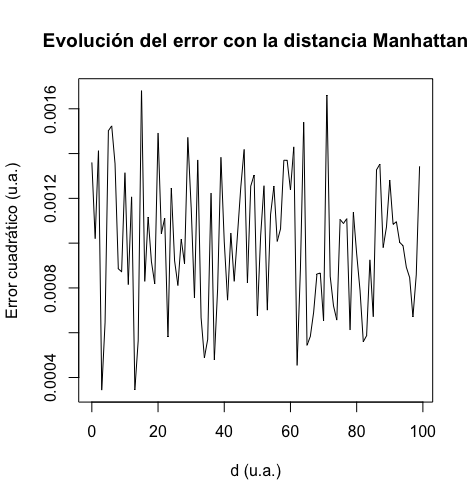
\includegraphics[width=7truecm]{Rplotmanh.png}
%     \caption{Error en función de la distancia en unidades arbitrarias.}
%     \label{fig:my_label}
% \end{figure}

...


%%%%%%%%%%%%%%%%%%%%%%%%%%%%%%%%%%%%%%%%%%%%%%%%%%%%
% Tercera parte: Resultados + Discusión  <--> PEC3 %
%%%%%%%%%%%%%%%%%%%%%%%%%%%%%%%%%%%%%%%%%%%%%%%%%%%%


\chapter{Discusión}
\label{chap:Discusión}

% Discusión de los resultados en el contexto del proyecto. Es en este apartado donde cobran sentido y en el cual se responden las preguntas de investigación y se muestra cómo los resultados dan respuesta a los problemas planteados.

...


%%%%%%%%%%%%%%%%%%%%%%%%%%%%%%%%%%%%%%%%%%%%%%%%%%%%%%%%%%%%%%%%%%%%%%%%%%%%%
% Cuarta parte: Conclusión + Retoques (Glosario, seguimiento...)  <--> PEC4 %
%%%%%%%%%%%%%%%%%%%%%%%%%%%%%%%%%%%%%%%%%%%%%%%%%%%%%%%%%%%%%%%%%%%%%%%%%%%%%


\chapter{Conclusiones y trabajos futuros}
\label{chap:Conclusiones y trabajos futuros}

\section{Conclusiones}
\label{sec:Conclusiones}

% Este capítulo tiene que incluir:
% 
% \begin{itemize}
% \item Una descripción de las conclusiones del trabajo:
% \begin{itemize}
%     \item Una vez se han obtenido los resultados, ¿qué conclusiones se extraen?
%     \item ¿Estos resultados son los esperados? ¿O han sido sorprendentes? ¿Por qué?
% \end{itemize}
% \item Una reflexión crítica sobre el logro de los objetivos planteados inicialmente:
% \begin{itemize}
%     \item ¿Hemos logrado todos los objetivos? Si la respuesta es negativa, ¿por qué motivo?
% \end{itemize}
% \end{itemize}

...


\section{Líneas de futuro}
\label{sec:Líneas de futuro}

% Las líneas de trabajo futuro que no se han podido explorar en este trabajo y han quedado pendientes.

...


\section{Seguimiento de la planificación}
\label{sec:Seguimiento de la planificación}

% \begin{itemize}
% \item
% Un análisis crítico del seguimiento de la planificación y metodología a lo largo del producto:
% \begin{itemize}
%     \item ¿Se ha seguido la planificación?
%     \item ¿La metodología prevista ha sido suficientemente adecuada?
%     \item ¿Ha habido que introducir cambios para garantizar el éxito del trabajo? ¿Por qué?
% \end{itemize}
% \item De los impactos previstos a \ref{s:etic}, ético-sociales, de sostenibilidad y de diversidad, avaluad/mencionad si se han mitigado (si eran negativos) o si se han conseguido (si eran positivos).
% \item Si han aparecido impactos no previstos en \ref{s:etic}, evaluar/mencionar cómo se han mitigado (si eran negativos) o que han aportado (si eran positivos).
% \end{itemize}

...


\newpage
\scriptsize

% Antes de \printglossaries especificar el estilo (list, altlist, listgroup, listhypergroup)
% \glossarystyle{list}
\printglossaries
% \printglossaries[type=\acronymtype]


\newpage
\scriptsize

\bibliographystyle{IEEEtran} % Opciones: abbrv, acm, alpha, apalike, ieeetr, plain, siam, unsrt
\bibliography{TFM}


%%%%%%%%%%%%%%%%%%%%%%%%
% Secciones opcionales %
%%%%%%%%%%%%%%%%%%%%%%%%


% \newpage
% 
% \appendix
% 
% %Listado de apartados que son demasiado extensos para incluir dentro de la memoria y tienen un carácter autocontenido (por ejemplo, manuales de usuario, manuales de instalación, etc.)
% 
% %Dependiendo del tipo de trabajo, es posible que no haya que añadir algún anexo.
% 
% \chapter{Anexo A}
% \label{chap:Anexo A}
% 
% \section{Anexo 1}
% \label{chap:Anexo 1}




% -------------------------------------------------------------------------------------------------------%
% -------------------------------------------------------------------------------------------------------%
% ----------------------------------- U  T  I  L  I  D  A  D  E  S --------------------------------------%
% -------------------------------------------------------------------------------------------------------%
% -------------------------------------------------------------------------------------------------------%

% %%%%%%%%%%%%%%%%%%%%%%%%%%%%%%
% % Para introducir ecuaciones %
% %%%%%%%%%%%%%%%%%%%%%%%%%%%%%%
% 
% % Introducir una ecuación numerada y con etiqueta:
% % ------------------------------------------------
% 
% \begin{equation}\label{eq:etiquetaEq}
% Eq
% \end{equation}
% \myequations{Descripción Eq}
% 
% % Referenciar una ecuación:
% % -------------------------
% 
% La ecuación ~\ref{eq:etiquetaEq} es ...
% 
% % Poner paréntesis alrededor de una referencia de ecuación:
% % ---------------------------------------------------------
% 
% La ecuación \eqref{eq:pythagoras} es ...
% 
% % Para introducir ecuaciones no numeradas:
% % ----------------------------------------
% 
% \begin{equation*}
% Eq
% end{equation*}
% \myequations{Descripción Eq}
% 
% % Para introducir ecuaciones con diversas fórmulas:
% % -------------------------------------------------
% 
% \begin{align}
% e^{i\pi} & = \cos(\pi) + i\sin(\pi) \notag \\
%          & = -1 .
% \end{align}
% 
% \begin{equation}
%     1 + 1 = 2
% \end{equation}
% \label{eq:2.1}


% -------------------------------------------------------------------------------------------------------%


\end{document}
